\capitulo{5}{Resultados}
En esta sección se presentan los resultados obtenidos mediante la simulación de los modelos SI, SIS, SIR y SEIR, tanto en sus versiones básicas como con vacunación, utilizando Simulink. 

Es importante destacar que el parámetro $\beta$ que se emplea en los modelos corresponde a la tasa de transmisión ajustada o efectiva, aque para simplificar a partir de ahora se denominará solo beta, aunque sea la efectiva.

\section{Comportamiento modelo SI}
Para el modelo SI se han realizado tres simulaciones con distintos valores de $\beta$ y condiciones iniciales, tal como se resume en la Tabla \ref{tab:resultadosSI}. Estas simulaciones permiten analizar cómo varía la propagación de una infección.
\begin{table}[H]
\centering
\begin{tabular}{|c|c|c|}
\hline
\textbf{Parámetro} & \textbf{Suimulación 1} & \textbf{Simulación 2}  \\
\hline
Susceptibles (S)  & 9990 & 9990 \\
\hline
Infectados (I)   & 10   & 10   \\
\hline
\(\beta\)       & 0.000001 & 0.00008 \\
\hline
\end{tabular}
\caption{Datos usados para ver el comportamiento del modelo SI.}
\label{tab:resultadosSI}
\end{table}
A continuación, se presentan los resultados de cada simulación en la figura (\ref{fig:comparacion_SI}).
Como se puede observar, independientemente del valor de $\beta$, todos los individuos susceptibles acaban infectándose con el paso del tiempo. La tasa de transmisión únicamente influye en la velocidad a la que se propaga la infección, pero no en el resultado final.


\begin{figure}[htbp]
    \centering
    \begin{subfigure}[b]{0.9\linewidth}
        \centering
        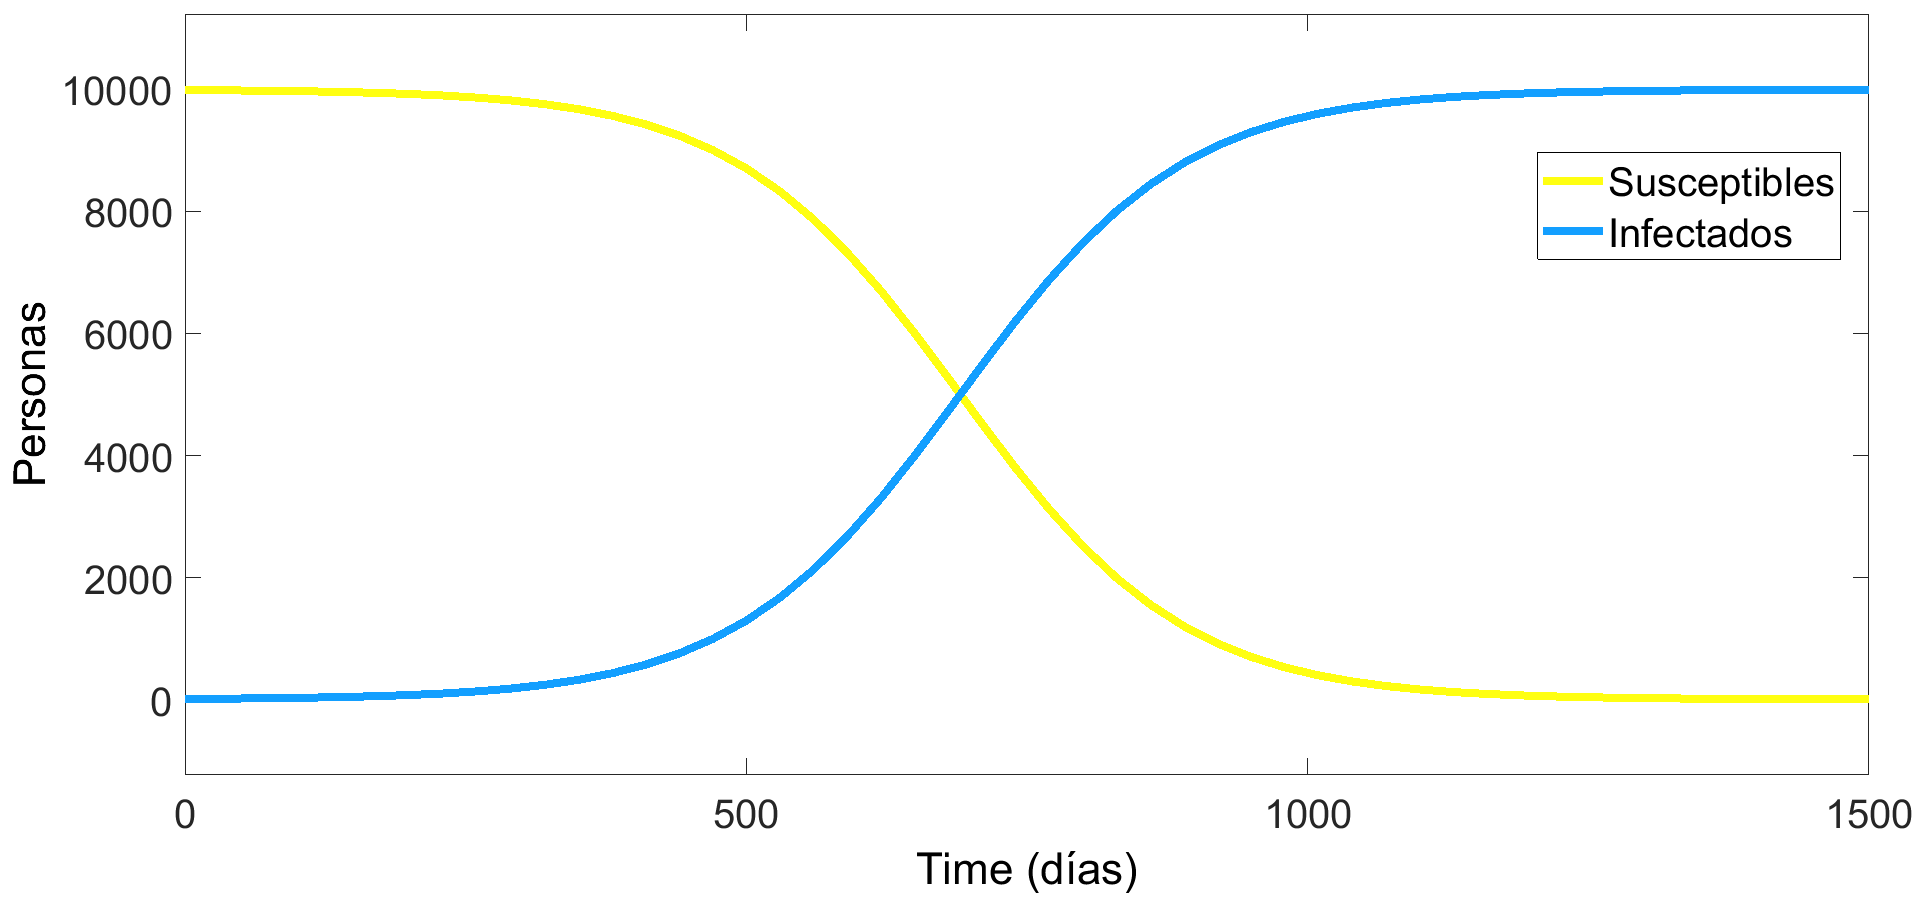
\includegraphics[width=\linewidth]{img/modelo SI 0.000001.png}
        \caption{Resultado del modelo SI con $\beta = 0{,}000001$.}
        \label{fig:simulacion_2_SI}
    \end{subfigure}
    
    \vspace{0.5cm}
    
    \begin{subfigure}[b]{0.9\linewidth}
        \centering
        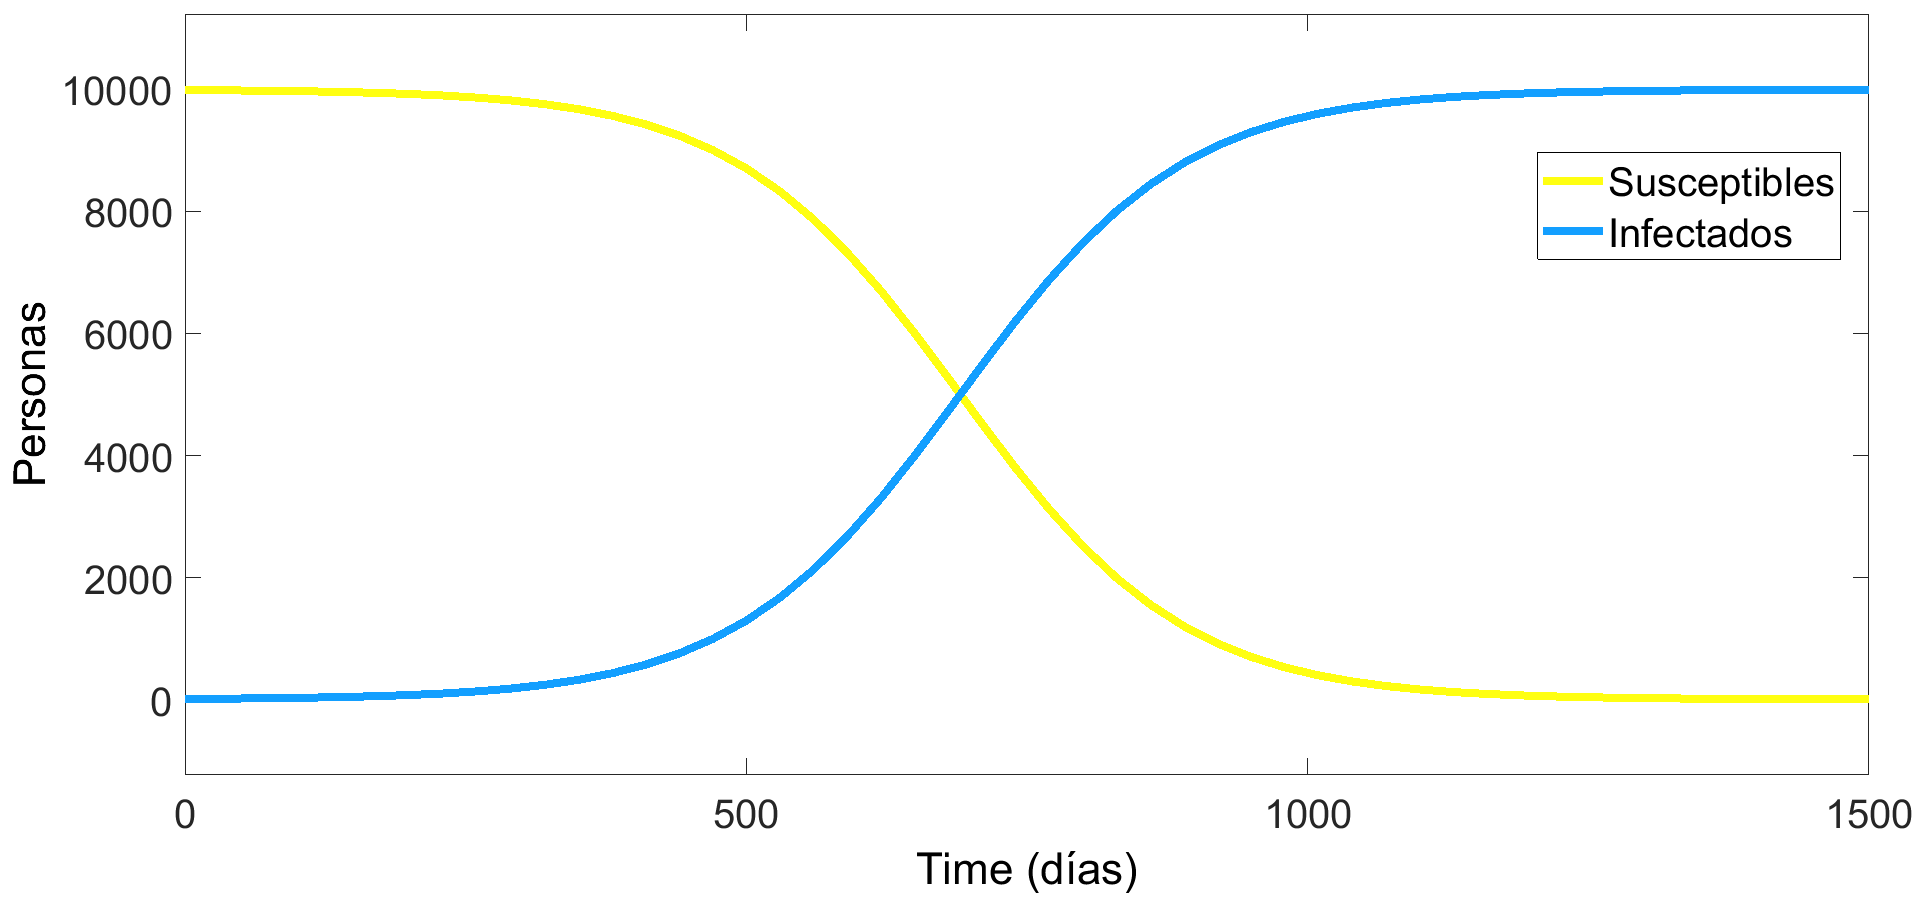
\includegraphics[width=\linewidth]{img/modelo SI 0.000001.png}
        \caption{Resultado del modelo SI con $\beta = 0{,}00008$.}
        \label{fig:simulacion_3_SI}
    \end{subfigure}
    
    \caption{Comparación de la evolución del modelo SI con distintos valores del parámetro $\beta$.}
    \label{fig:comparacion_SI}
\end{figure}





 


\subsection{Comportamiento epidemia SIDA/VIH}
A continuación, se presenta la simulación del comportamiento de la epidemia del VIH/SIDA, utilizando los parámetros definidos anteriormente en el apartado de descripción de los datos. La figura \ref{fig:vih} muestra la evolución de la enfermedad a lo largo del tiempo, destacando cómo se comporta la dinámica de contagio bajo el modelo utilizado.

Tras simularlo la grafica \ref{fig:vih} muestra la evolución de la enfermedad en la región MENA a lo largo de un periodo de 365 días, utilizando el modelo SI con los parámetros definidos previamente.
La línea amarilla representa el número de personas susceptibles, mientras que a línea azul muestra el número de personas infectadas, aquellas que han adquirido la enfermedad y permanecen en este estado, no hay recuperación.
Al principio de la simulación, casi toda la población es susceptible y solo una pequeña parte se encuentra infectada. Sin embargo, debido a la tasa de transmisión $\beta$, se observa un crecimiento exponencial del número de infectados.
Hacia el día 70, la curva de infectados y la de susceptibles se cruzan, la mayoría de la población ya está infectada. Finalmente, la curva de personas infectadas se estabiliza en el total de la población, mientras que la de susceptibles en cero.

\begin{figure}[htbp]
    \centering
    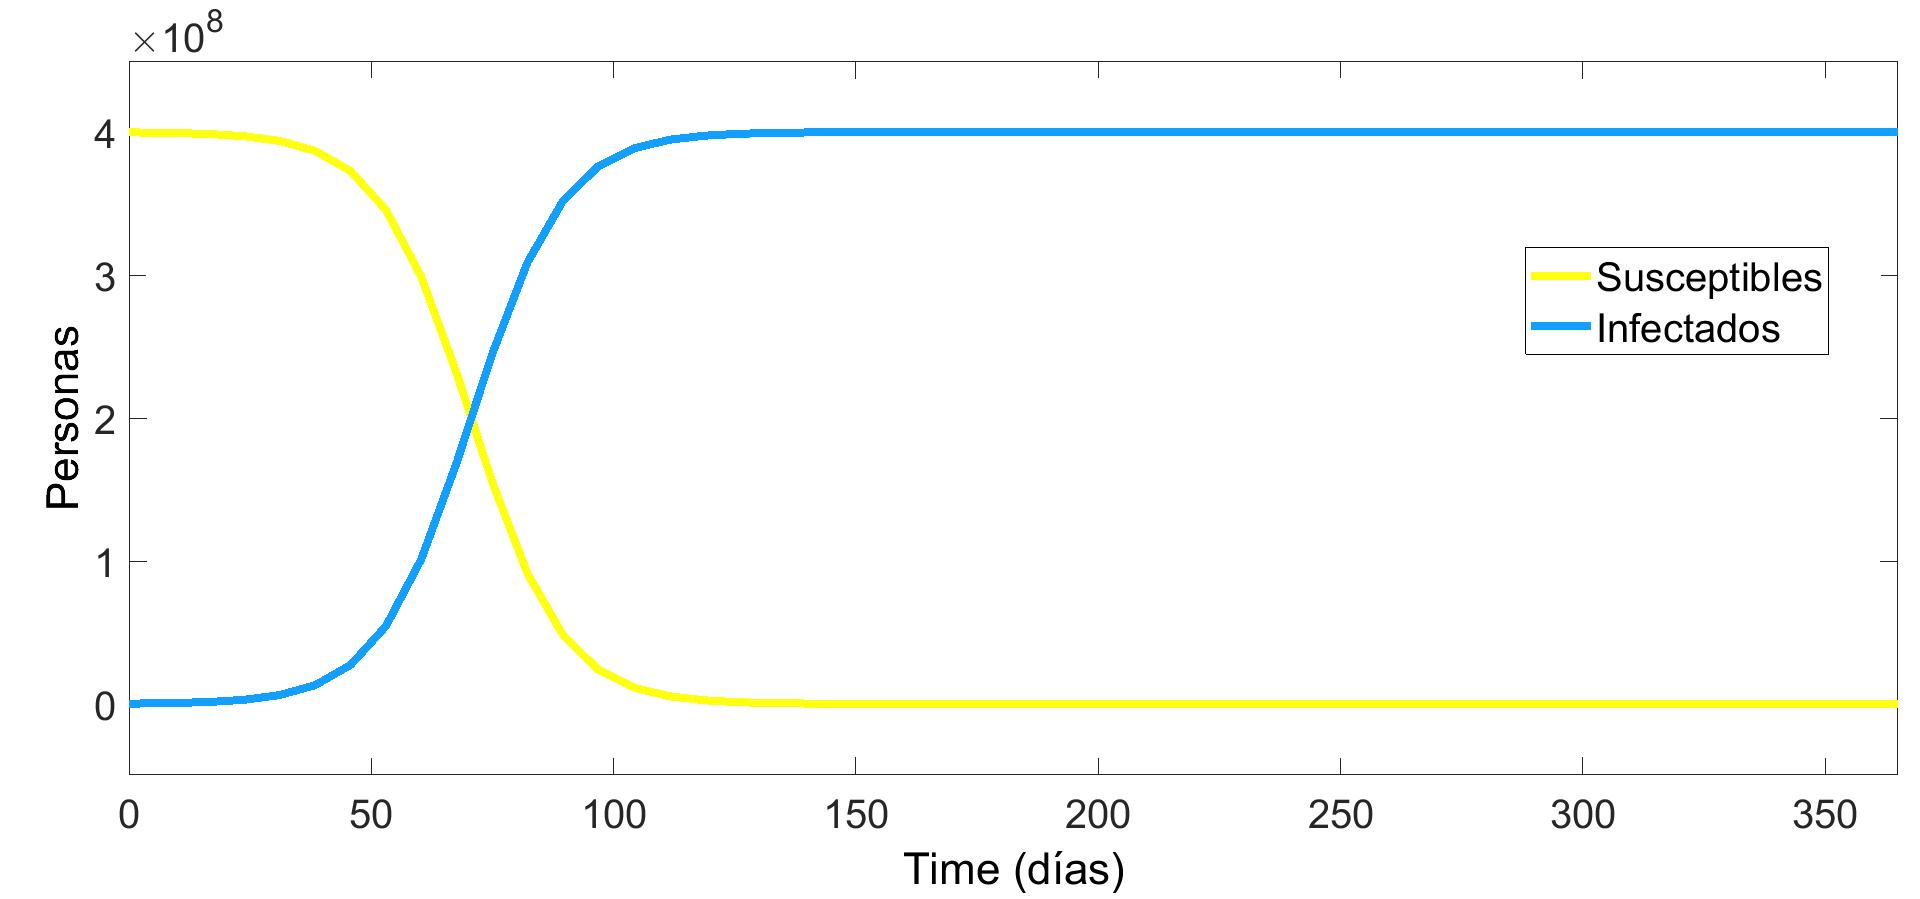
\includegraphics[width=0.9\textwidth]{img/modelo SI.jpg}
    \caption{Resultado modelo SI con los datos reales para el VIH/SIDA}
    \label{fig:vih}
    
\end{figure}





\section{Comportamiento modelo SIS}
Para el modelo SIS se han realizado simulaciones con distintos
valores para los parámetros como para las condiciones iniciales. Los datos utilizados se representan en la tabla \ref{tab:datos para modelo SIS}.
\begin{table}[H]
\centering
\begin{tabular}{|c|c|c|c|}
\hline
\textbf{Parámetro} & \textbf{Simulación 1} & \textbf{Simulación 2}  \\
\hline
Susceptibles (S)  & 8000 & 8000\\
\hline
Infectados (I)      & 2000 & 2000  \\
\hline
\(\beta\)         & 0.0000002  & 0.00007\\
\hline
\(\gamma\)        & 0.3 & 0.15\\
\hline
$R_0$         &   0.006     &  4,6    \\
\hline
\end{tabular}
\caption{Datos usados para ver el comportamiento del modelo SIS.}
\label{tab:datos para modelo SIS}
\end{table}

En la Figura~\ref{fig:simulacion2_SIS}, los infectados disminuyen rápidamente hasta desaparecer, mientras los susceptibles vuelven a representar la totalidad de la población. Esto indica una erradicación completa de la enfermedad, alcanzando un estado libre de infección gracias a un número básico de reproducción $R_0 < 1$.
Por el contrario, en la Figura~\ref{fig:simulacion3_SIS}, la enfermedad no desaparece, sino que se mantiene de forma persistente en la población. El sistema alcanza un equilibrio dinámico en el que el número de infectados y susceptibles permanece constante en el tiempo. Este comportamiento es característico de enfermedades endémicas, donde $R_0 > 1$, permitiendo la transmisión continua sin que la infección desaparezca por completo.

\begin{figure}[H]
    \begin{subfigure}[b]{0.9\linewidth}
        \centering
        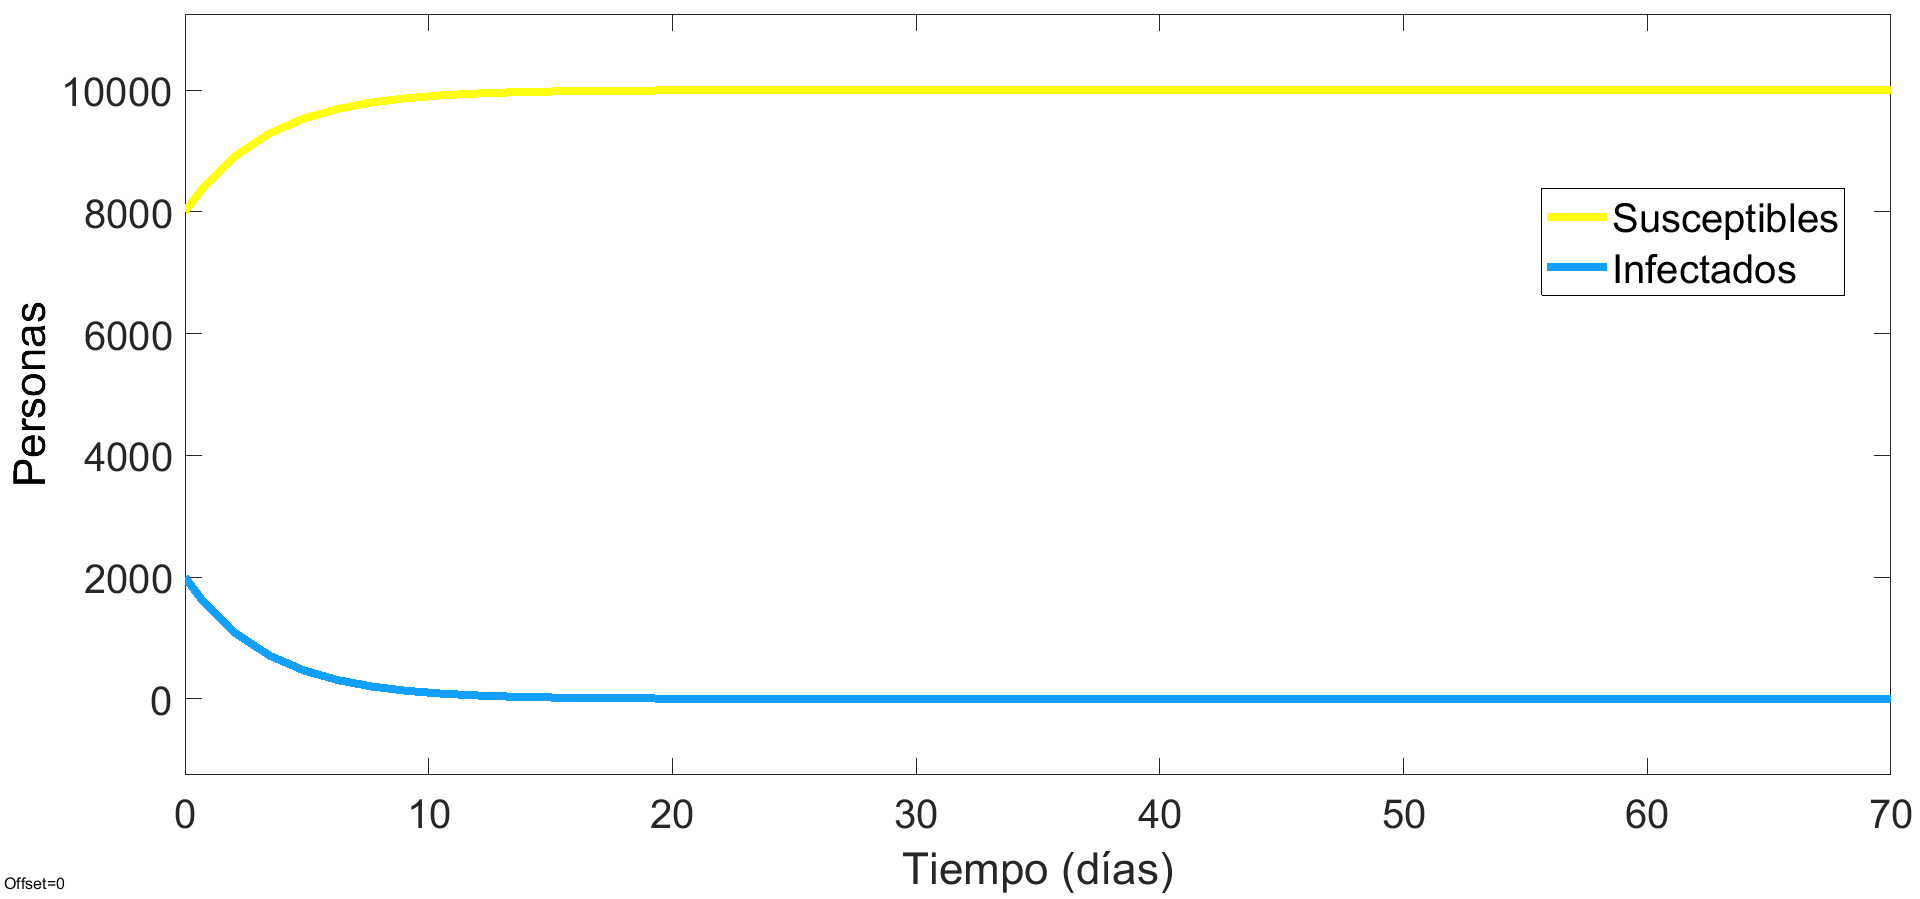
\includegraphics[width=\linewidth]{img/modelo SIS23.png}
        \caption{Resultado del modelo SIS con $\beta = 0{,}0000002$ y $\gamma = 0{,}3$.}
        \label{fig:simulacion2_SIS}
    \end{subfigure}
    
    \vspace{0.5cm}

    \begin{subfigure}[b]{0.9\linewidth}
        \centering
        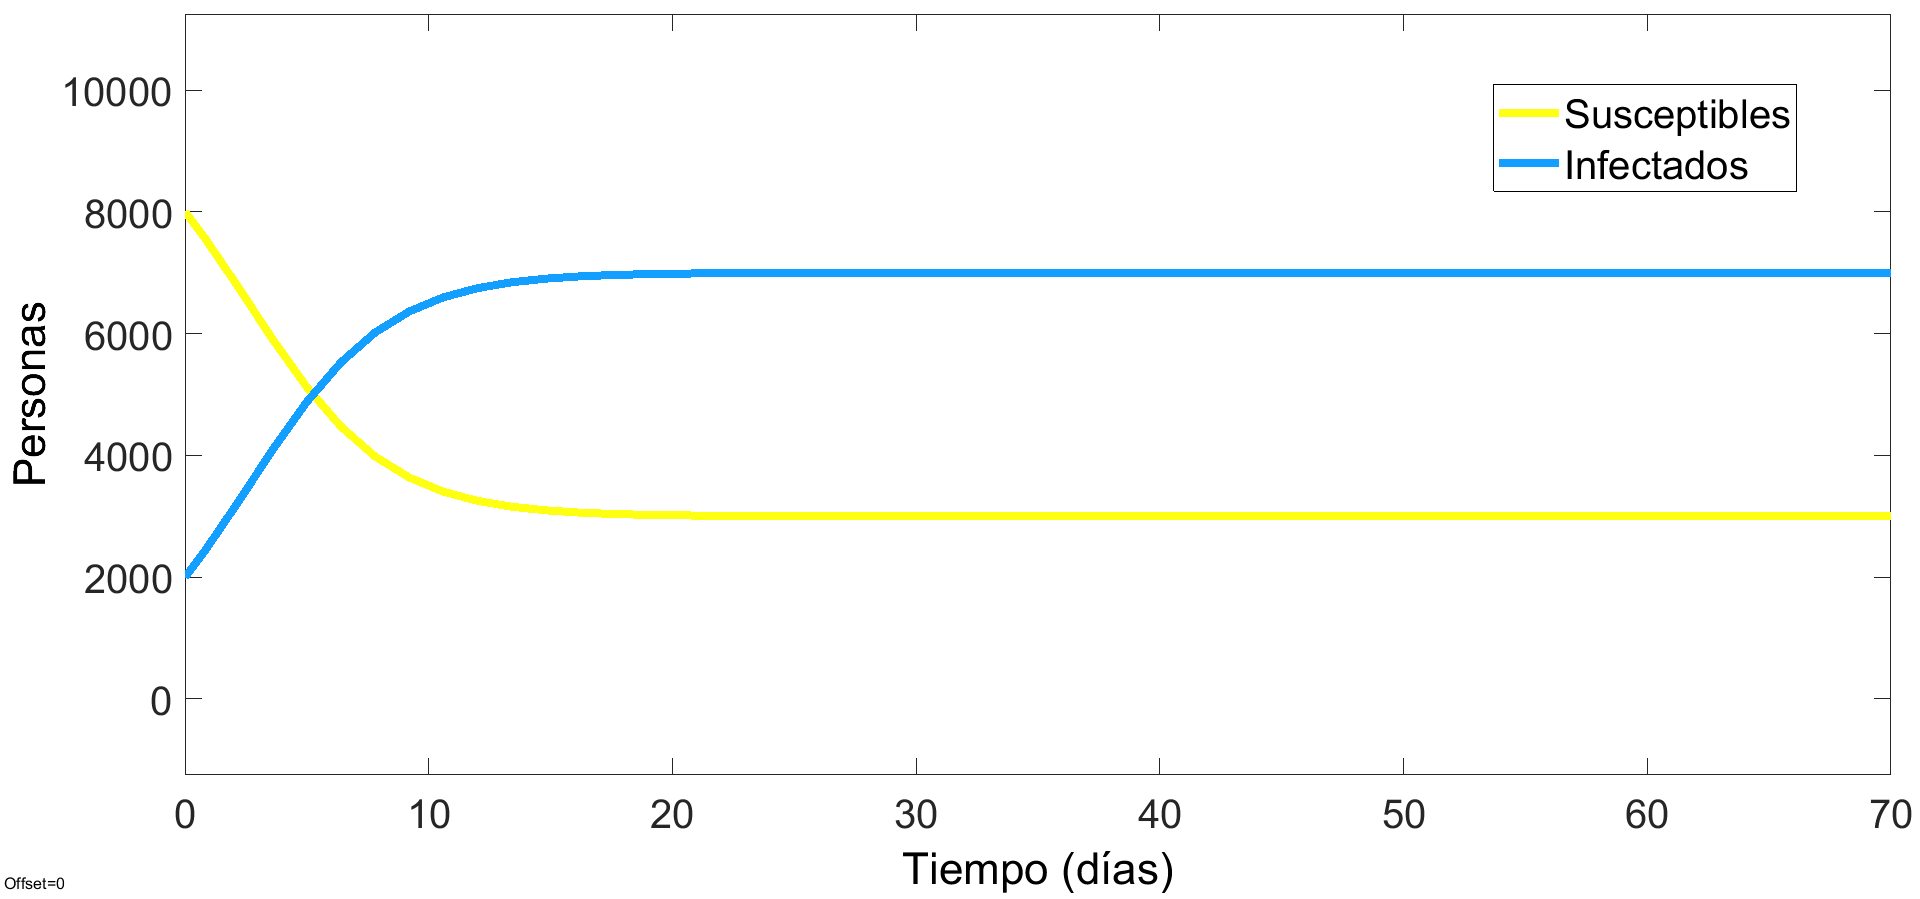
\includegraphics[width=\linewidth]{img/modelo SIS b0.5 g0.15.png}
        \caption{Resultado del modelo SIS con $\beta = 0{,}00007$ y $\gamma = 0{,}15$.}
        \label{fig:simulacion3_SIS}
    \end{subfigure}

    \caption{Comparación del comportamiento del modelo SIS con distintos valores de $\beta$ y $\gamma$.}
    \label{fig:comparacion_SIS}
\end{figure}





\subsection{Comportamiento epidemia gonorrea}
A continuación, se presenta  la simulación del comportamiento de la epidemia de la gonorrea, utilizando los parámetros definidos anteriormente en el apartado de descripción de los datos. La figura \ref{fig:simugono} muestra la evolución de la enfermedad a lo largodel tiempo, destacando la dinámica de contagio bajo el modelo utilizado.

\begin{figure}[H]
    \centering
    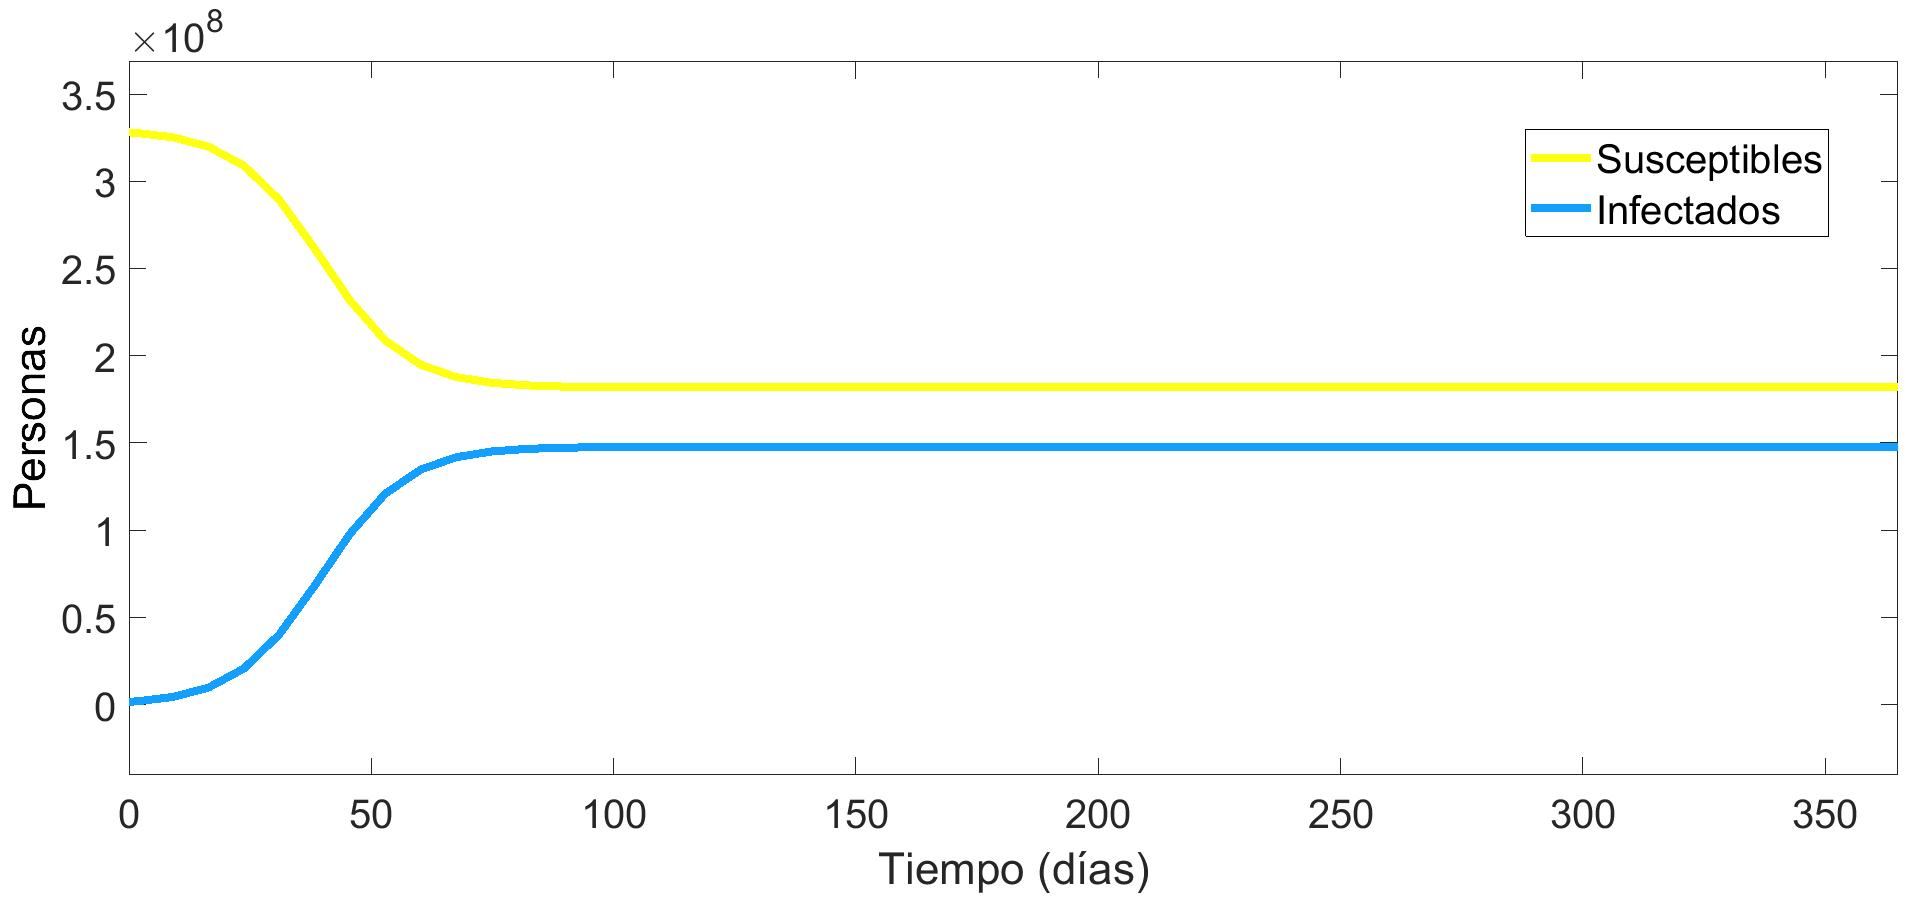
\includegraphics[width=0.9\textwidth]{img/modelo SIS.jpg}
    \caption{Resultado modelo SIS con los datos reales para la gonorrea}
    \label{fig:simugono}
    
\end{figure}

La gráfica obtenida \ref{fig:simugono} tras simular el modelo SIS muestra la evolución temporal de la infección a lo largo de un año. Se observa que inicialmente el número de infectados crece de forma acelerada, mientras que la cantidad de individuos susceptibles disminuye de manera brusca. Esta fase inicial refleja el momento en el que la transmisión domina sobre la recuperación, debido a la elevada proporción de individuos susceptibles y la presencia activa de personas infectadas.
Conforme transcurren los días, la velocidad de crecimiento de la infección disminuye y ambas curvas comienzan a estabilizarse. Esto indica que el sistema alcanza un equilibrio epidemiológico estable, característico del modelo SIS, en el que el número de nuevas infecciones diarias se compensa con el número de recuperaciones. Dado que los individuos recuperados no adquieren inmunidad y vuelven al compartimento de susceptibles, la enfermedad no desaparece, sino que persiste con una proporción constante de la población infectada.
Se calcula el número básico de reproducción en la ecuación \eqref{eq:R0_179}.
\begin{equation}
R_0 = \frac{\beta}{\gamma} = \frac{0.25}{0.14} \approx 1{,}79
\label{eq:R0_179}
\end{equation}
Lo que significa que de media cada persona infectada contagiará aproximadamente a 1,79 personas al día mientras este infectada. Como este valor es mayor que uno, se cumple la condición para que la infección se propague en la población y no desaparezca, como se observa en el resultado de la gráfica. Esto implica que los individuos pueden volver a infectarse. El $R_0$ > 1 indica que la tasa de nuevas infecciones supera a la tasa de recuperaciones, y que la enfermedad se propagará hasta que se alcance un equilibrio endémico. En este equilibrio, la proporción de personas infectadas y susceptibles se mantiene constante en el tiempo.





\section{Comportamiento modelo SIR}
Para el modelo SIR se han realizado varias simulaciones con valores distintos para las condiciones iniciales y parámetros. Los datos que se utilizan se encuentran en la tabla \ref{tab:datos para modelo SIR}.
\begin{table}[H]
\centering
\begin{tabular}{|c|c|c|}
\hline
\textbf{Parámetro} & \textbf{Simulación 1} & \textbf{Simulación 2}  \\
\hline
Susceptibles (S) & 8000 & 8000 \\
\hline
Infectados (I)   & 2000   & 2000   \\
\hline
Recuperados (R)   &  0   & 0   \\
\hline
\(\beta\)        & 0.000007 & 0.0000002  \\
\hline
\(\gamma\)        & 0.01 & 0.4 \\
\hline
$R_0$      &     7   &    0.005       \\
\hline
\end{tabular}
\caption{Datos usados para ver el comportamiento del modelo SIR}
\label{tab:datos para modelo SIR}
\end{table}

Se observan los resultados para cada simulación en la figura \ref{fig:comparacion_SIR}. En la Figura~\ref{fig:simulacion1_SIR}, la enfermedad se propaga lentamente pero de forma generalizada. Todos los susceptibles acaban infectados y posteriormente recuperados. El pico de infecciones se alcanza alrededor del día 100 con aproximadamente 6000 casos. El número básico de reproducción, $R_0$, en este caso es 7, lo que explica la rápida expansión del brote. Finalmente, la epidemia se extingue al no quedar individuos susceptibles.
En la Figura~\ref{fig:simulacion2_SIR}, la enfermedad apenas logra propagarse. Los infectados iniciales se recuperan rápidamente, y la mayoría de la población permanece susceptible sin experimentar nuevos contagios significativos. Aquí, $R_0 < 1$, lo que indica que cada infectado contagia a menos de una persona, lo cual impide que el brote se mantenga. Esta simulación muestra cómo el valor de $R_0$ determina si una epidemia se expande o se extingue rápidamente.

\begin{figure}[H]
    \centering

    \begin{subfigure}[b]{0.9\linewidth}
        \centering
        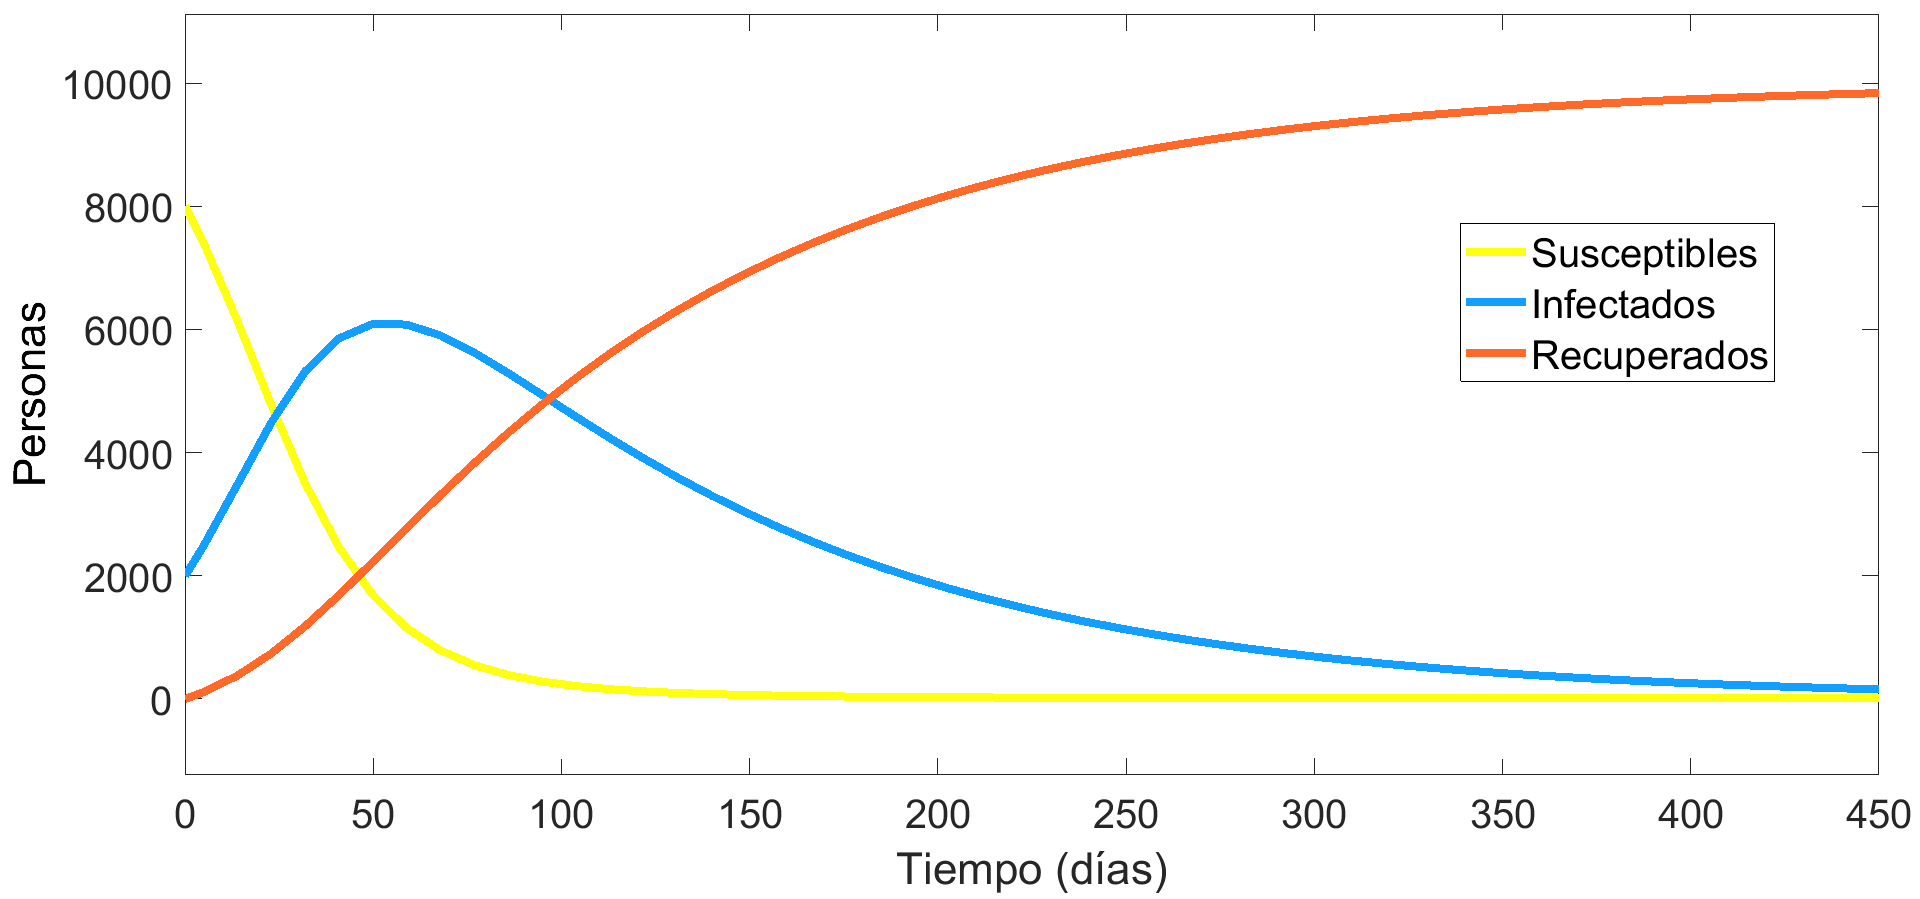
\includegraphics[width=\linewidth]{img/modelo SIR b0.000007 g0.1.png}
        \caption{Resultado del modelo SIR con $\beta = 0{,}000007$ y $\gamma = 0{,}01$.}
        \label{fig:simulacion1_SIR}
    \end{subfigure}

    \vspace{0.5cm}

    \begin{subfigure}[b]{0.9\linewidth}
        \centering
        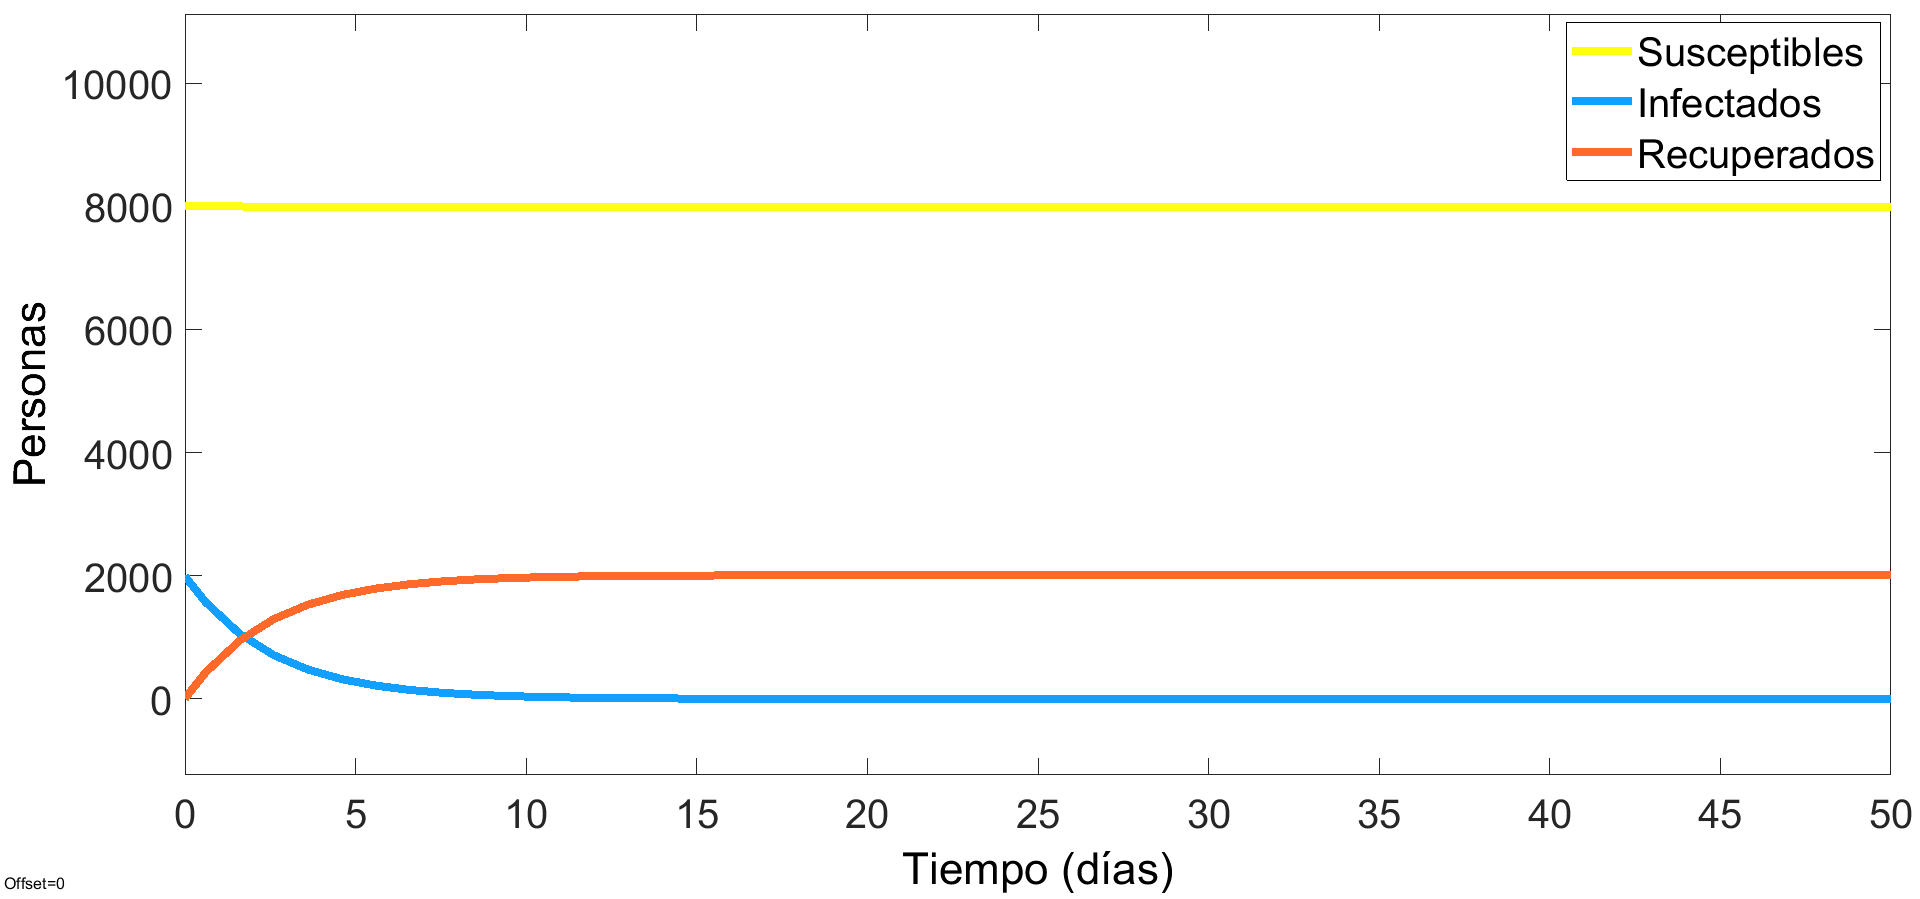
\includegraphics[width=\linewidth]{img/modelo SIR b0.0000002 g0.4.png}
        \caption{Resultado del modelo SIR con $\beta = 0{,}0002$ y $\gamma = 0{,}4$.}
        \label{fig:simulacion2_SIR}
    \end{subfigure}

    \caption{Comparación del modelo SIR con distintos valores de $\beta$ y $\gamma$.}
    \label{fig:comparacion_SIR}
\end{figure}










\subsection{Comportamiento epidemia sarampión}
Se simula el comportamiento de la enfermedad del sarampión, utilizando los datos definidos anteriormente en el apartado de descripción de los datos. La figura \ref{fig:simusara} muestra la evolución del sarampión. Se refleja claramente el comportamiento típico de una enfermedad infecciosa altamente contagiosa, y más si no hay medidas de control como la vacuna.
Al principio, la mayor parte de la población se encuentra en el grupo de susceptibles. Sin embargo, debido al gran valor de $R_0$, la enfermedad se propaga con rapidez. Como consecuencia los susceptibles descienden bruscamente en los primero días, un gran número de personas contrae la enfermedad en un corto periodo de tiempo. Posteriormente, la curva llega a cero, que refleja que toda la población se ha infectado.
En cuanto a los infectados, la curva presenta un crecimiento rápido al principio de la epidemia, alcanzando un pico endémico sobre el día 12. En este punto se registra el número máximo de personas infectadas de forma simultánea. Tras este pico, los infectados empiezan a disminuir progresivamente. Esto es debido a que las personas se recuperan y pasan al compartimento de los recuperados, y además quedan muy pocos susceptibles, por lo que la transmisión se ralentiza hasta que se detiene.
Por otro lado, los recuperados van creciendo sostenidamente en el tiempo, empezando en cero y creciendo de forma acelerada en un principio. A medida que los infectados se recuperan, la curva sube hasta que toda la población ha superado la enfermedad y ha adquirido inmunidad permanente. Cuando la curva de los recuperados se estabiliza indica que la epidemia ha llegado a su fin, porque no quedan personas susceptibles que puedan volver a infectarse.

\begin{figure}[H]
    \centering
    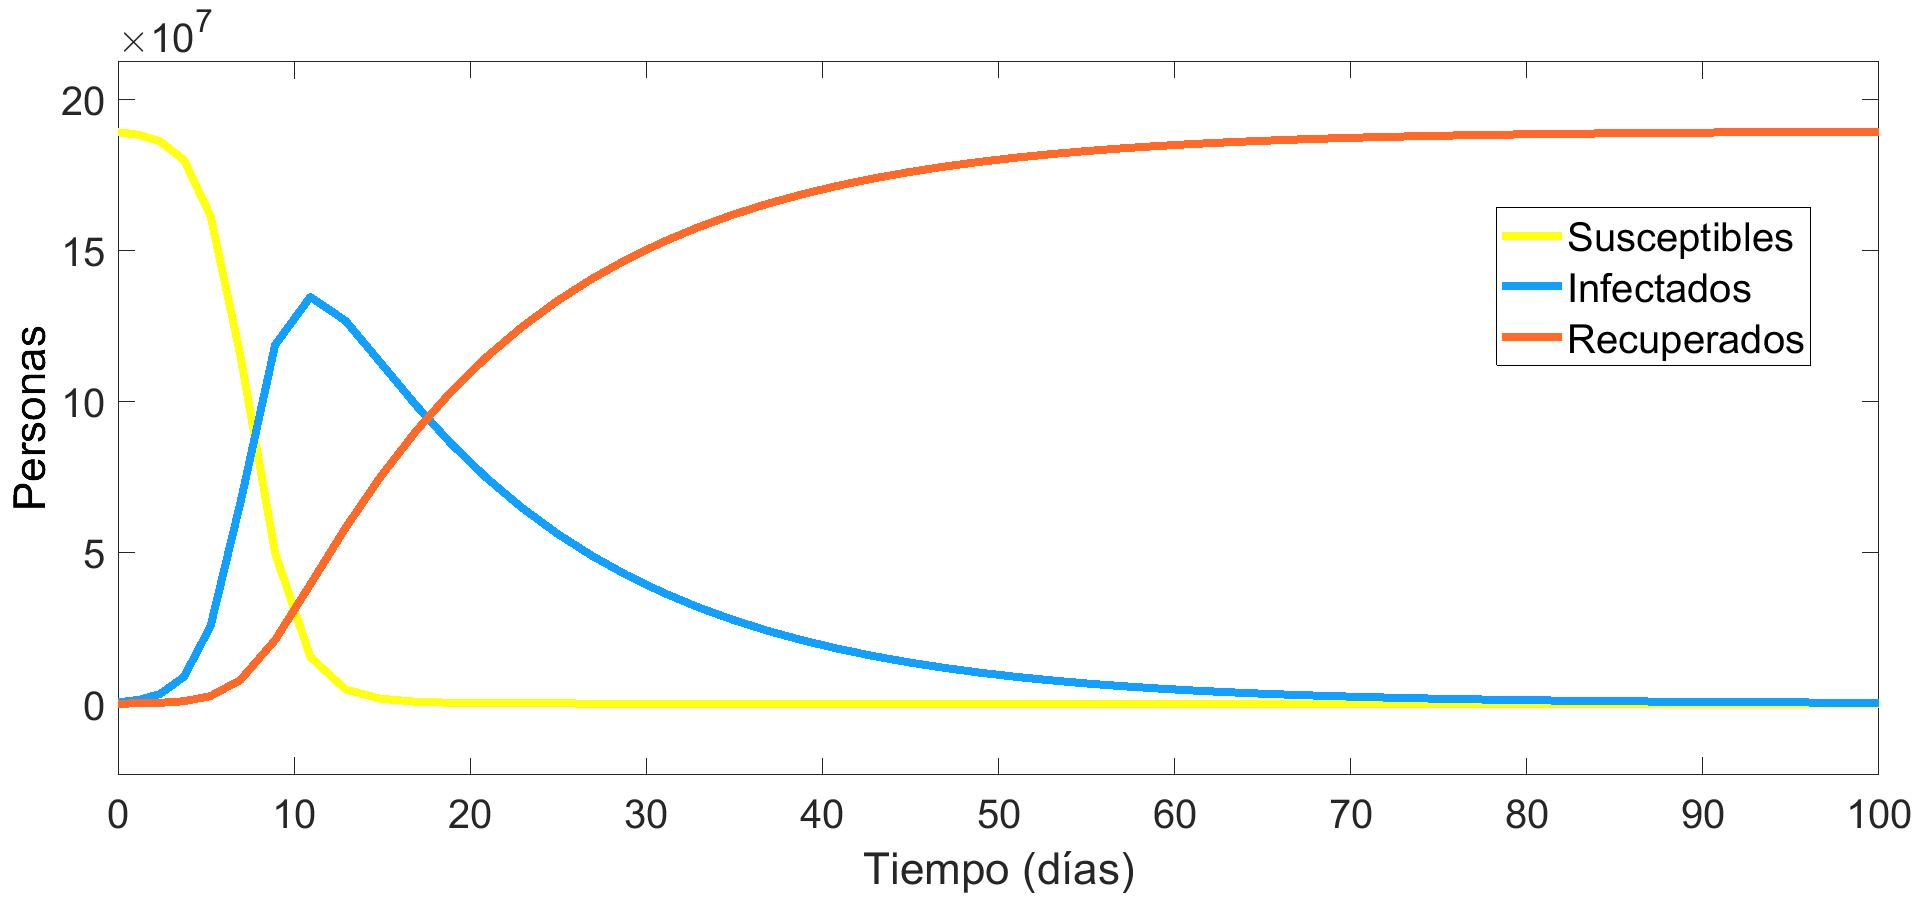
\includegraphics[width=0.9\textwidth]{img/modelo SIR.jpg}
    \caption{Resultado modelo SIR con datos reales para el sarampión}
    \label{fig:simusara}
    
\end{figure}







\section{Comportamiento modelo SEIR}
Para el modelo SEIR se han realizado varias simulaciones con valores distintos. Los datos que se utilizan se encuentran en la tabla \ref{tab:datos para modelo SEIR} y los resultados en la figura \ref{fig:comparacion_SEIR}.

\begin{table}[H]
\centering
\begin{tabular}{|c|c|c|}
\hline
\textbf{Parámetro} & \textbf{Simulación 1} & \textbf{Simulación 2}  \\
\hline
Susceptibles (S) & 8000 & 8000 \\
\hline
Expuestos (R)   &  0   & 0   \\
\hline
Infectados (I)   & 2000   & 2000   \\
\hline
Recuperados (R)   &  0   & 0   \\
\hline
\(\beta\)        & 0.000007 & 0.0000002  \\
\hline
\(\sigma\)        & 0.1 & 0.2  \\
\hline
\(\gamma\)        & 0.01 & 0.4\\
\hline
\end{tabular}
\caption{Datos usados para ver el comportamiento del modelo SEIR}
\label{tab:datos para modelo SEIR}
\end{table}





\begin{figure}[H]
    \centering

    \begin{subfigure}[b]{0.9\linewidth}
        \centering
        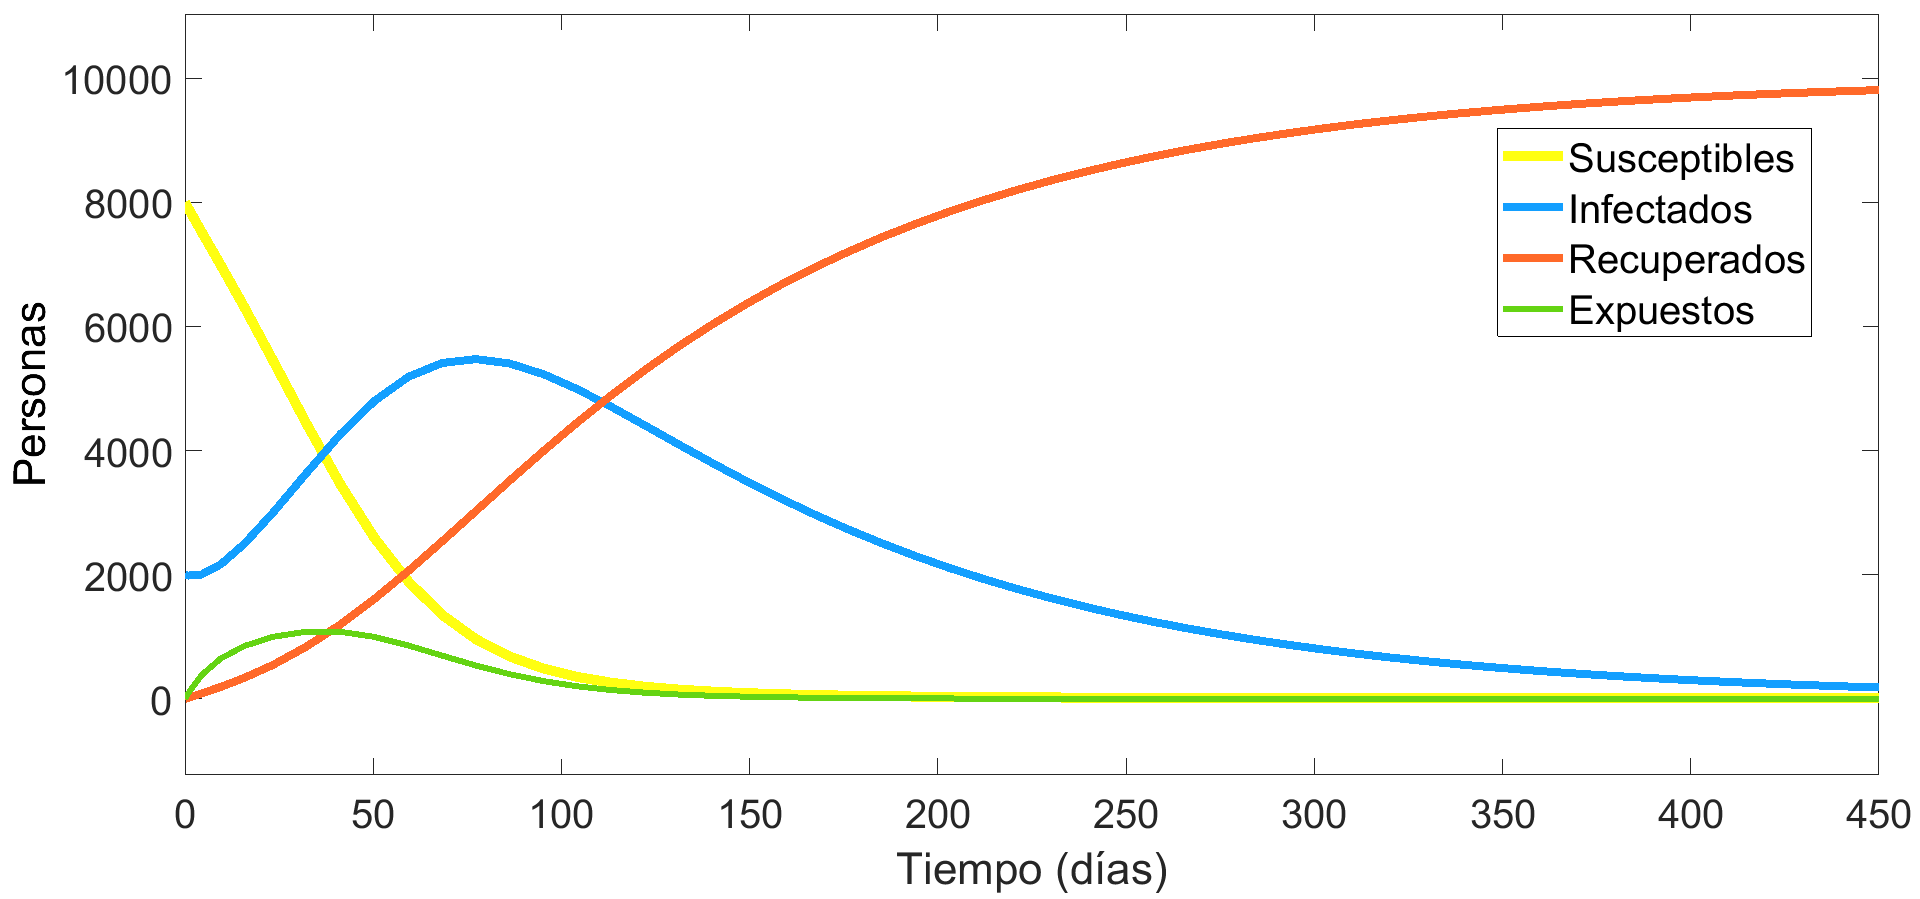
\includegraphics[width=\linewidth]{img/modelo SEIR b0.7 s0.1 g0.01.png}
        \caption{Resultado del modelo SEIR con $\beta = 0{,}000007$ y $\gamma = 0{,}01$.}
        \label{fig:simulacion1_SEIR}
    \end{subfigure}

    \vspace{0.5cm}

    \begin{subfigure}[b]{0.9\linewidth}
        \centering
        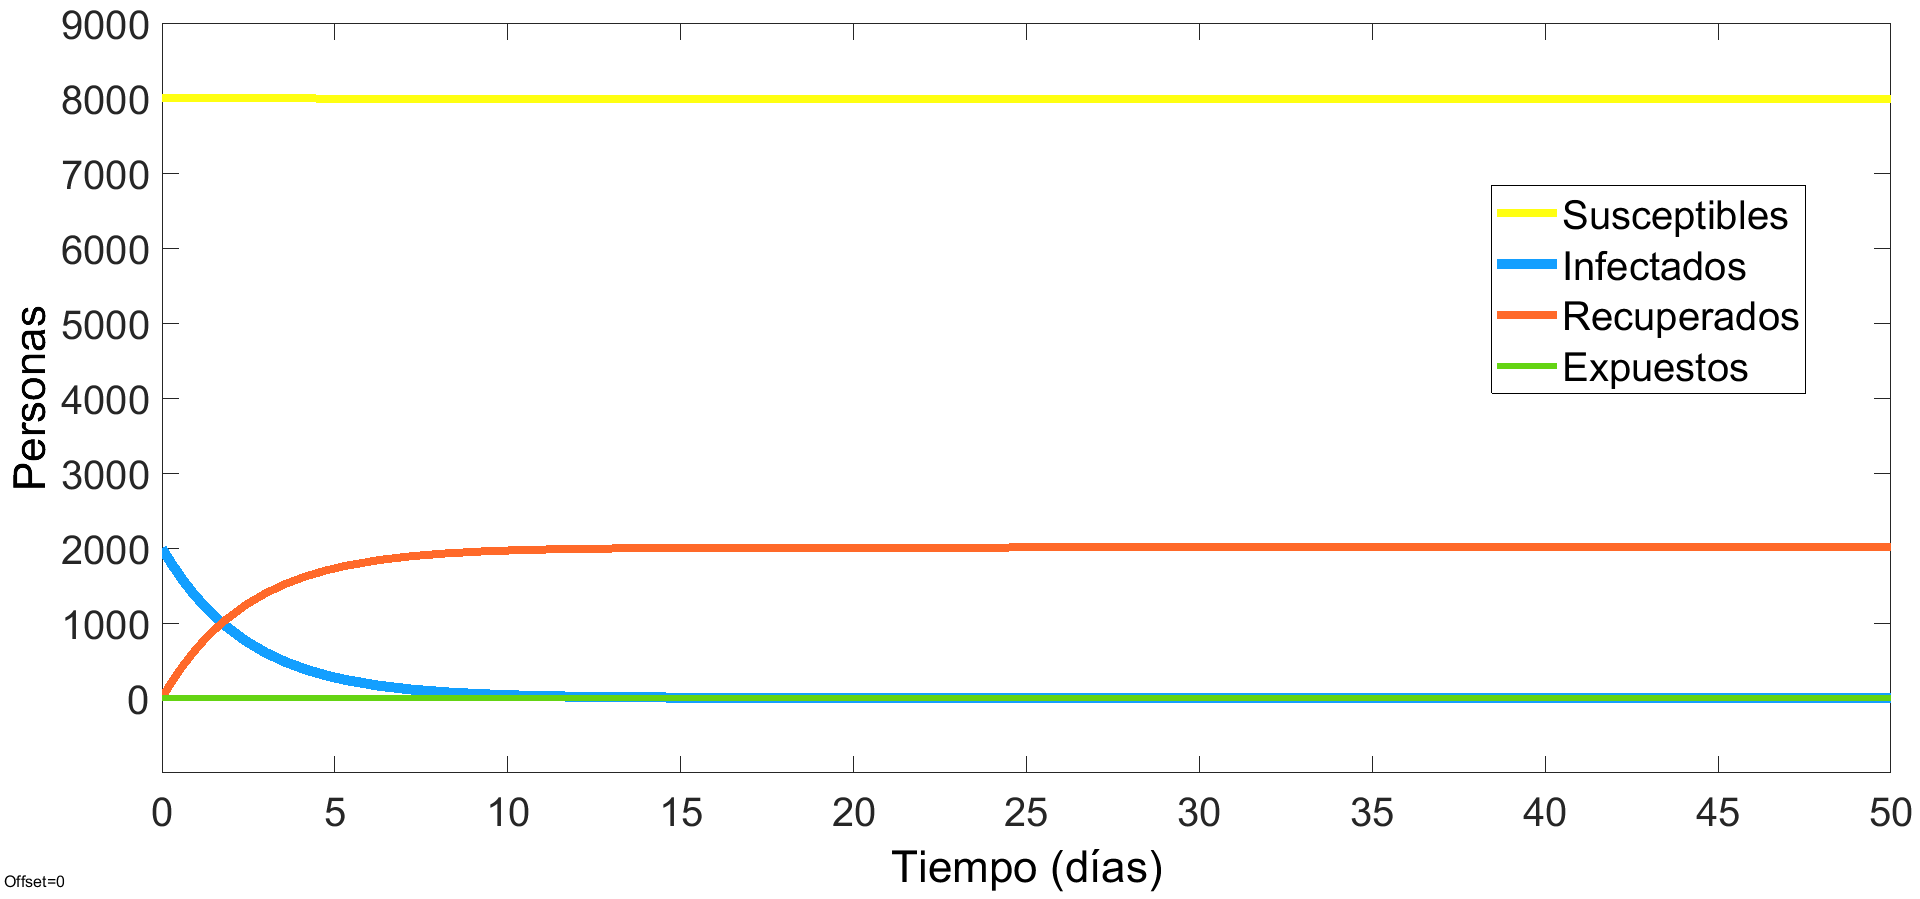
\includegraphics[width=\linewidth]{img/modelo seir b0.02 s0.2 g0.4.png}
        \caption{Resultado del modelo SEIR con $\beta = 0{,}0002$ y $\gamma = 0{,}4$.}
        \label{fig:simulacion2_SEIR}
    \end{subfigure}

    \caption{Comparación del modelo SEIR con distintos valores de $\beta$ y $\gamma$.}
    \label{fig:comparacion_SEIR}
\end{figure}

En la Figura~\ref{fig:simulacion1_SEIR}, el número de personas expuestas crece inicialmente y luego decrece. Los infectados presentan un pico moderado, debido a la baja tasa de transmisión y a la recuperación lenta. Los recuperados aumentan paulatinamente, y los susceptibles disminuyen de forma progresiva, indicando una propagación lenta del brote.
En cambio, en la Figura~\ref{fig:simulacion2_SEIR}, la dinámica cambia drásticamente. Debido a que el valor de $\beta$ es mucho mayor que el de $\gamma$, el número de infectados alcanza un pico alto en poco tiempo. El brote es más explosivo, con una propagación rápida que genera un elevado número de infectados. La mayoría de la población pasa a la categoría de recuperados en un corto periodo, y los susceptibles se reducen drásticamente.




\subsection{Comportamiento pandemia COVID-19}
Se simula el comportamiento de la enfermedad del sarampión, utilizando los datos definidos anteriormente en el apartado de descripción de los datos. La figura \ref{fig:Simucov} muestra la evolución del COVID-19 en España desde su inicio.

\begin{figure}[H]
    \centering
    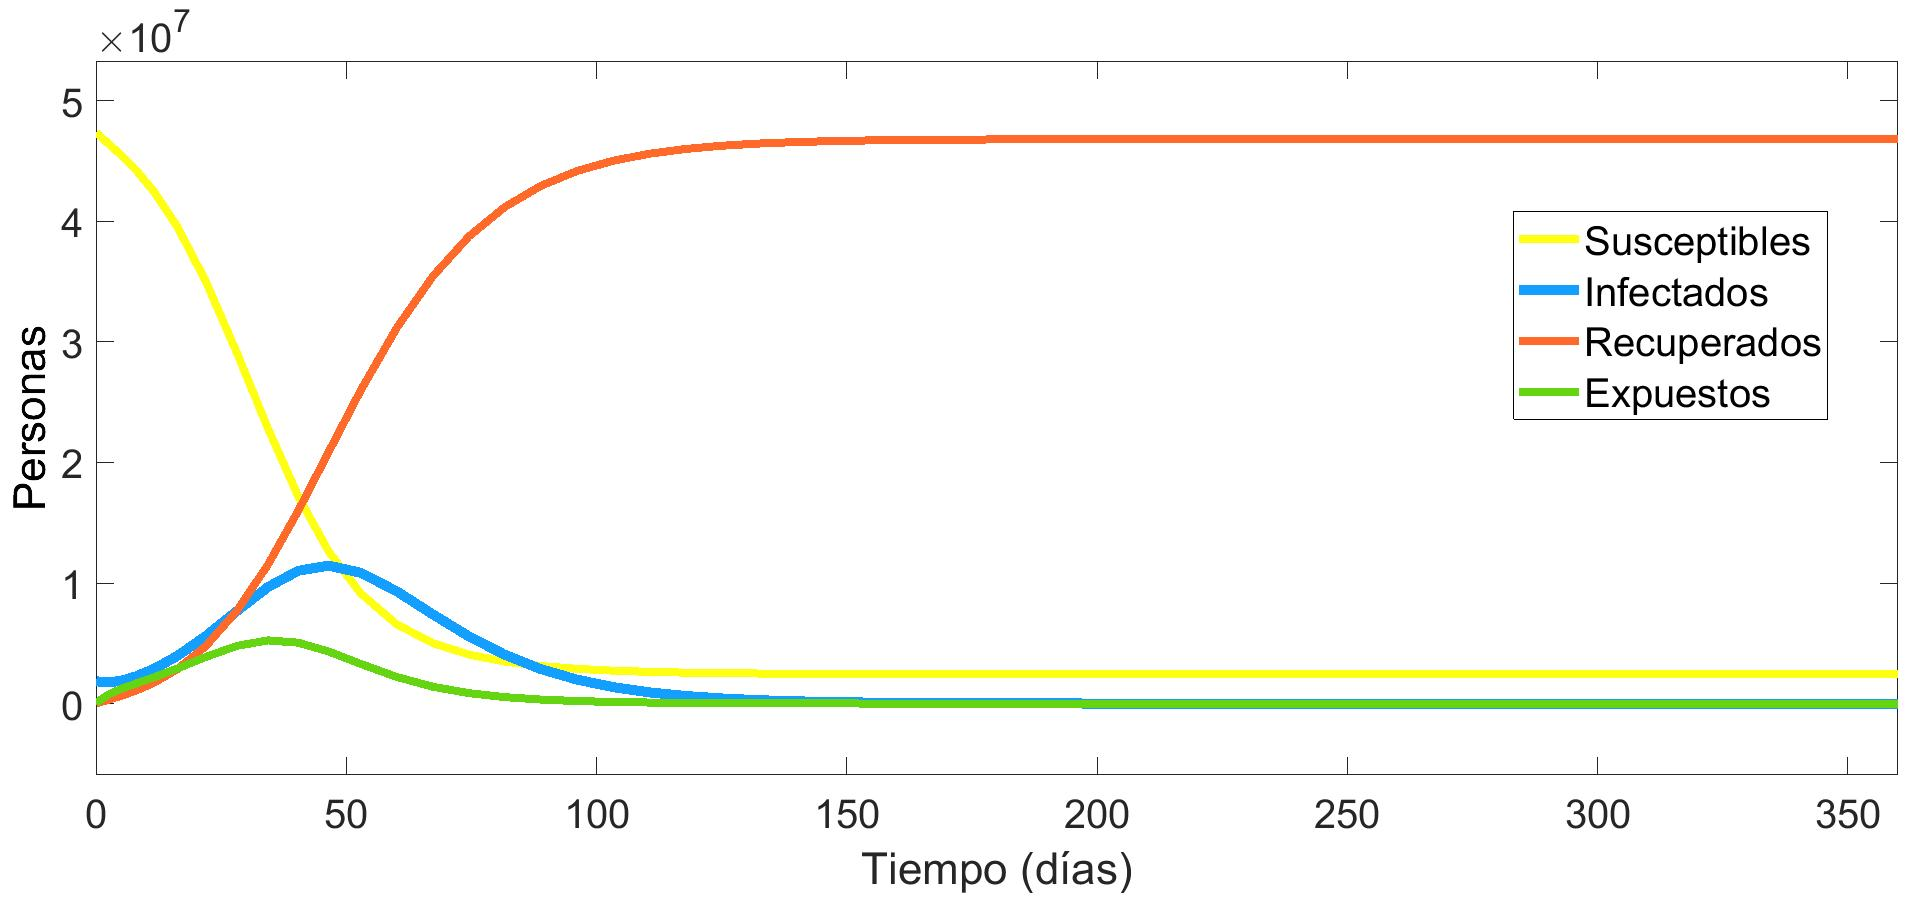
\includegraphics[width=0.9\textwidth]{img/modelo SEIR.jpg}
    \caption{Resultado modelo SEIR con datos reales para el COVID-19}
    \label{fig:Simucov}
    \vspace{0.5cm} % Ajusta el espacio vertical entre la imagen y el texto
\end{figure}

En la simulación \ref{fig:Simucov} se pueden obtener las siguientes observaciones. La población susceptible disminuye rápidamente, al inicio prácticamente la mayoría de la población era susceptible. mientras avanza el tiempo, disminuyen de manera pronunciada, debido al contacto entre las personas debido al contacto entre personas infectadas. La curva se estabiliza, gran parte de la población se ha contagiado, pero siguen quedando personas susceptibles.
La curva de los expuestos presenta un crecimiento inicial que se adelanta a la curva de los infectados, lo cual es coherente con este modelo, ya que las personas primero pasan por el periodo de incubación antes de convertirse en transmisores activos. El pico de personas infectadas se alcanza alrededor del día 50 aproximadamente, en este momento se observa mayor número de casos activos simultáneos. La curva desciende ya que los infectados se recuperan y los susceptibles disminuyen.
La curva de los recuperados mantiene un crecimiento constante, que se acelera con el pico de infecciones. Hacia el final de la simulación, la mayoría de la población se encuentra en el compartimento de recuperados, indica que la enfermedad ha dejado de propagarse de forma activa por falta de individuos susceptibles.
Aproximadamente a partir del día 150, el sistema entra en una fase de estabilidad. Los valores de todos los compartimentos se estabilizan, y prácticamente no hay nuevos contagios.  La enfermedad ha agotado su capacidad de transmisión debido a que casi toda la población ha adquirido inmunidad.
El retraso entre las curvas de expuestos e infectados muestra claramente el efecto del periodo de latencia. Este desfase temporal tiene consecuencias importantes desde el punto de vista epidemiológico, ya que dificulta la detección temprana de brotes y puede permitir la transmisión antes de que se manifiesten los síntomas.




\section{Medidas de control}
\subsection{Comportamiento modelo SIR con regulador PID}
Con el objetivo de mejorar el control sobre lo representado por el modelo SIR, se propone la implementación de un controlador PID. Este controlador permitirá ajustar dinámicamente una variable de control, la tasa de transmisión, en función del error entre el número actual de individuos infectados y un valor deseado (setpoint), que en este caso será de 1000 infectados. Para el diseño y ajuste del PID, se utilizarán los datos obtenidos previamente a partir de las simulaciones realizadas con el modelo SIR estándar, sin control. Estos datos permitirán identificar el comportamiento del sistema y evaluar la efectividad del controlador en mantener el número de infectados cercano al valor establecido.

En la figura (\ref{fig:simulacion1_SIRPID}) se observan las simulaciones para el modelo SIR controlado con un regulador PID.
En la Figura~\ref{fig:simulacion2_SIRPID}, la propagación de la enfermedad es moderada, el número de infectados aumenta gradualmente, alcanza un máximo y desciende de forma progresiva. El regulador PID actúa suavemente, logrando mantener el número de infectados cerca del valor de consigna (setpoint), evitando picos excesivos.
En la figura~\ref{fig:SIR_PID_2}, se observa un escenario más agresivo. La infección se propaga rápidamente y alcanza un pico muy pronunciado en un corto período de tiempo. A pesar de la rapidez de propagación, el PID reduce rápidamente los infectados, estabilizando la curva tras el pico inicial. El sistema logra acercarse nuevamente al valor deseado tras una breve oscilación.


\begin{figure}[H]
    \centering

    \begin{subfigure}[b]{0.9\linewidth}
        \centering
        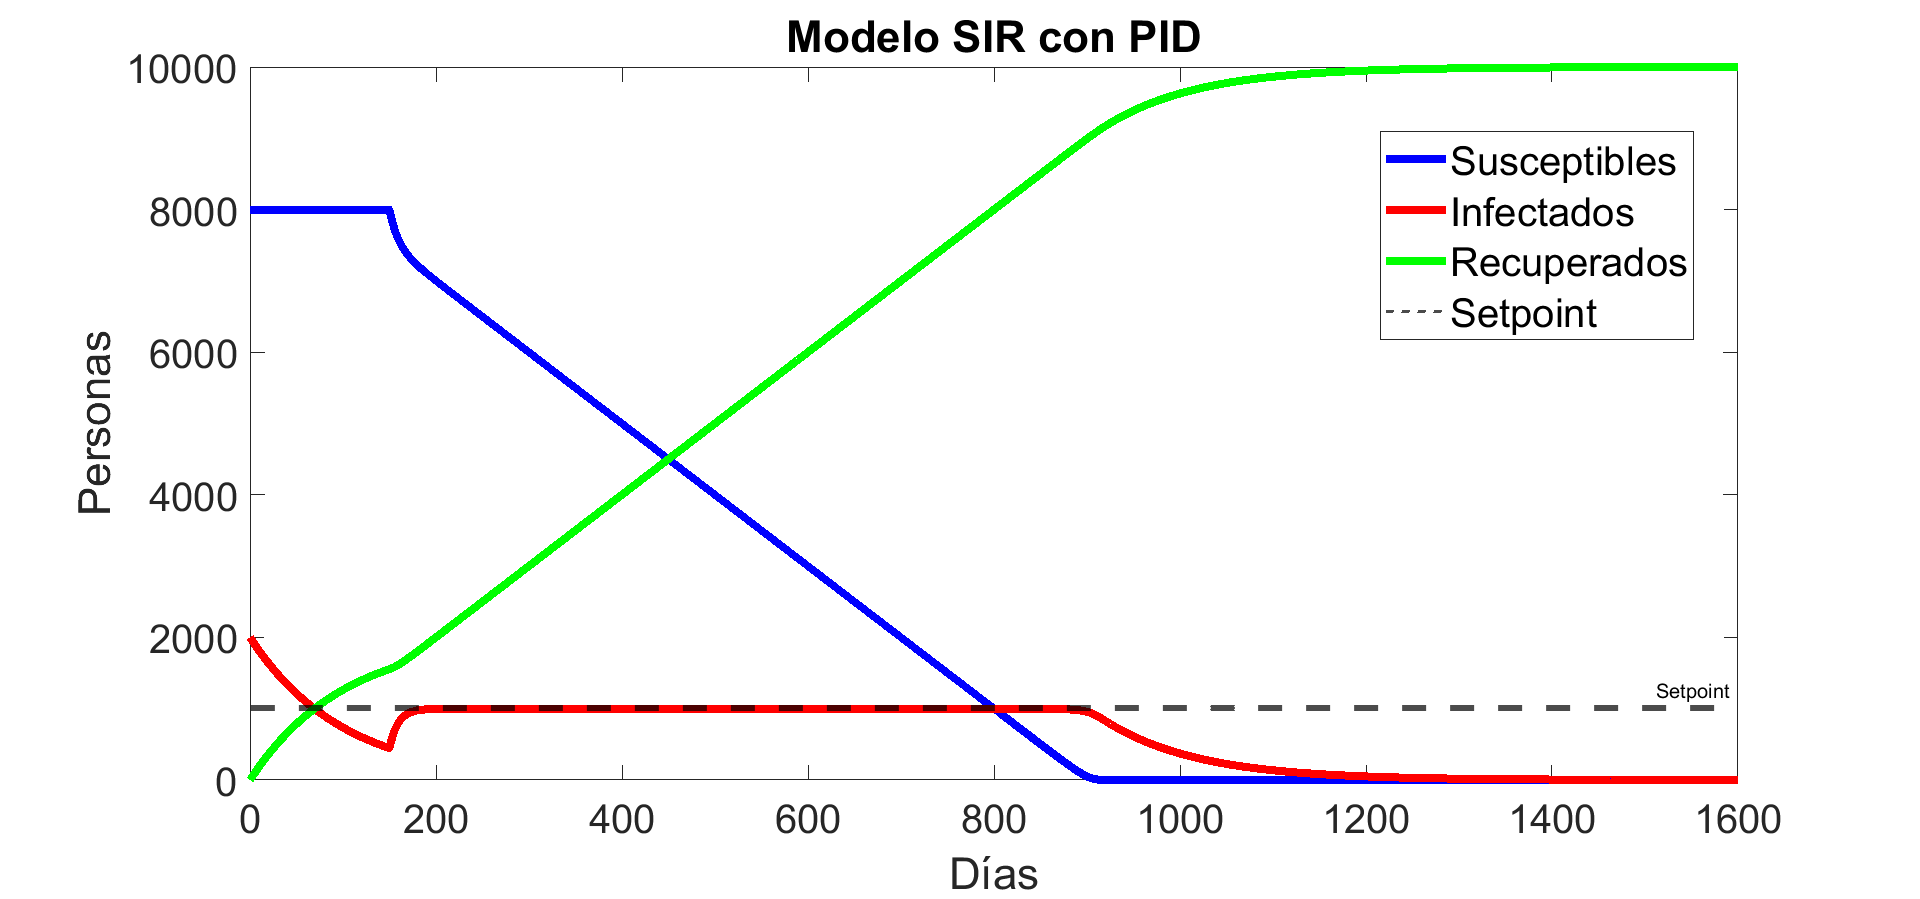
\includegraphics[width=\linewidth]{img/modelo SIR PID primera simulación.png}
        \caption{Resultado del modelo SIR con PID para los datos de la primera simulación de datos del modelo SIR.}
        \label{fig:simulacion1_SIRPID}
    \end{subfigure}

    \vspace{0.5cm}

    \begin{subfigure}[b]{0.9\linewidth}
        \centering
        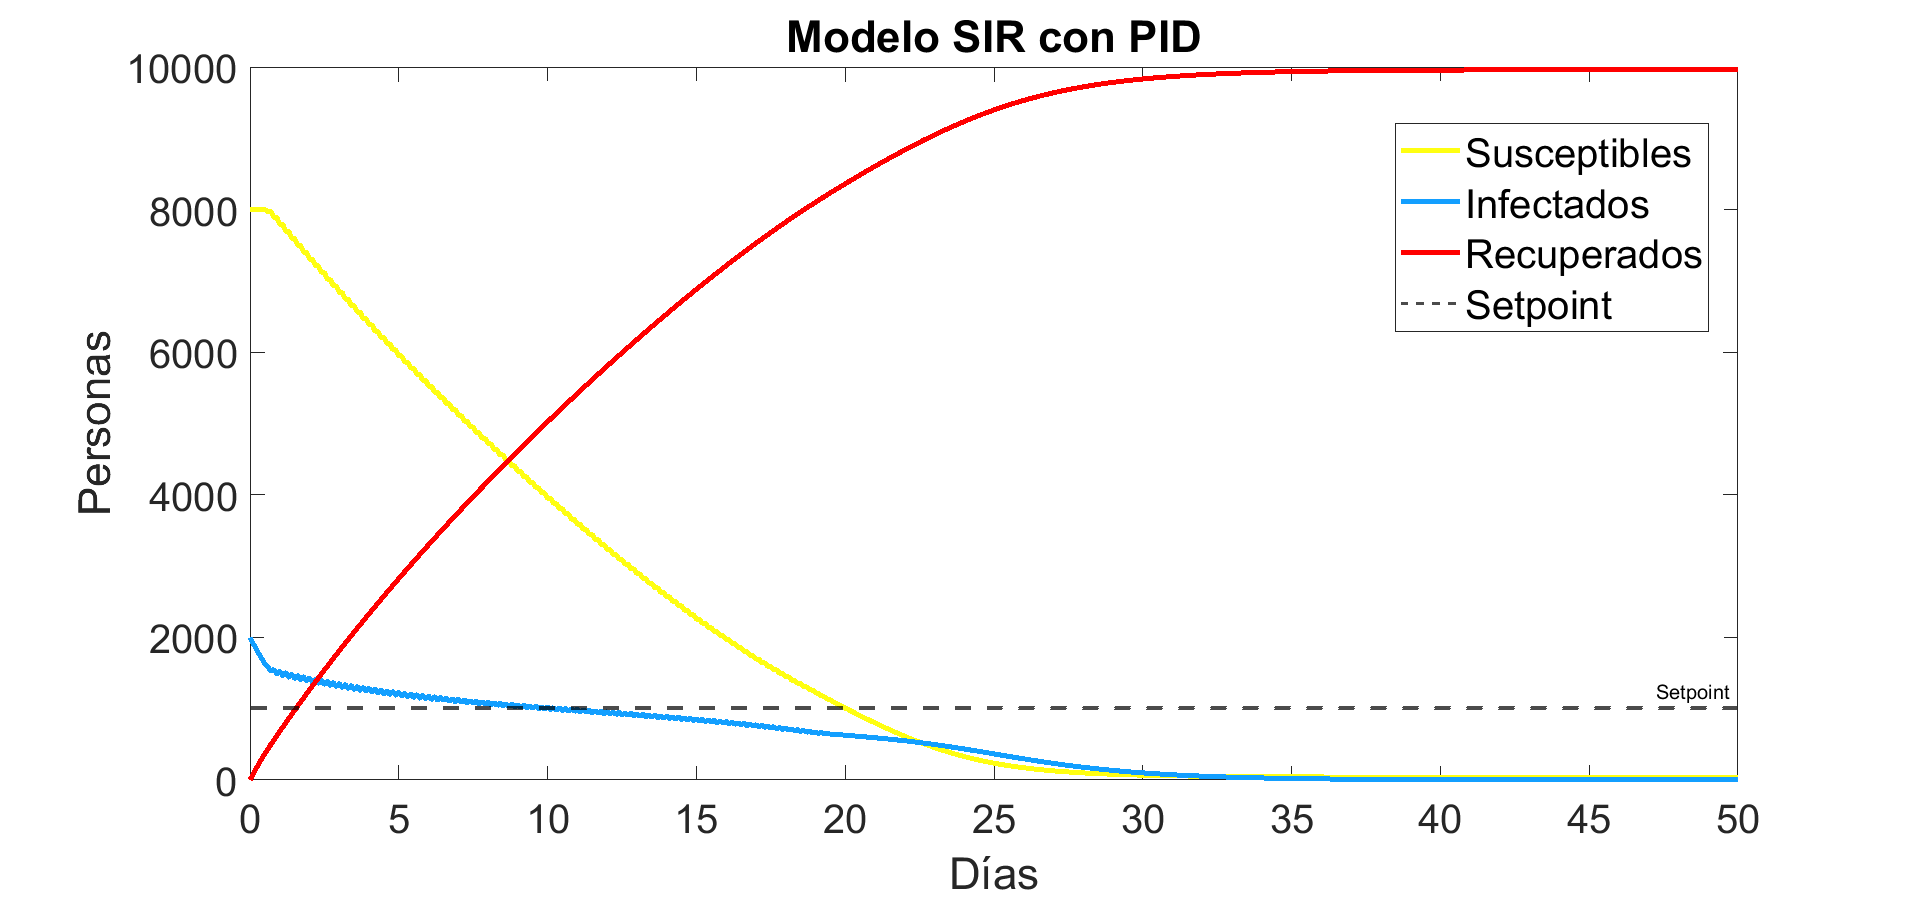
\includegraphics[width=\linewidth]{img/modelo SIR PID segunda simulacion.png}
        \caption{Resultado del modelo SIR con PID para los datos de la segunda simulación de datos del modelo SIR.}
        \label{fig:simulacion2_SIRPID}
    \end{subfigure}

    \caption{Comparación del modelo SIR con regulador PID para distintas simulaciones.}
    \label{fig:comparacion_SIRPID}
\end{figure}







\subsection{Comparación modelo SIR clásico y modelo SIR con regulador PID}


El modelo SIR clásico describe la evolución de una epidemia a partir de tres grupos poblacionales. Su comportamiento está determinado únicamente por los parámetros de transmisión y recuperación, por lo que no contempla mecanismos de intervención activa. La enfermedad suele seguir su curso natural: el número de infectados crece hasta alcanzar un pico, tras lo cual disminuye gradualmente a medida que los individuos se recuperan, dejando a la población con cierto grado de inmunidad o estabilidad.
Por otro lado, al incorporar un regulador PID al modelo SIR, se introduce un mecanismo de control que actúa sobre la dinámica del sistema en tiempo real. El controlador ajusta continuamente la tasa de contagio con el objetivo de mantener el número de infectados cerca de un valor de referencia o setpoint. Esta retroalimentación permite intervenir en el sistema antes de que el brote alcance niveles críticos.

Gracias a esta regulación, el modelo con PID presenta un comportamiento más eficiente desde el punto de vista del control epidemiológico. Se reduce el pico máximo de infectados, se acelera el proceso de recuperación y se acorta la duración total del brote. Además, el controlador puede evitar que la enfermedad se vuelva endémica, eliminando los casos activos incluso en escenarios donde el modelo clásico tendería a estabilizarse con una cantidad constante de infecciones.

El regulador PID dota al modelo SIR de una capacidad de respuesta activa, lo que permite contener la propagación de la enfermedad de forma más efectiva. Esta mejora es relevante para el diseño de estrategias de intervención en salud pública, ya que permite simular el impacto de medidas de control dinámicas como restricciones de movilidad, campañas de vacunación o medidas sanitarias adaptativas.

\subsection{Comportamiento del sarampión tras la vacunación}
Para este modelo, los datos también se han explicado en el apartado de descripción de los datos. Son los mismos que para sin vacunación, lo que pasa que se añade la tasa de vacunación ahora. La figura \ref{fig:simu saramp vacuna} muestra la evolución del sarampión pero contando que ahora se ha introducido como medida de control la vacunación.

\begin{figure}[H]
    \centering
    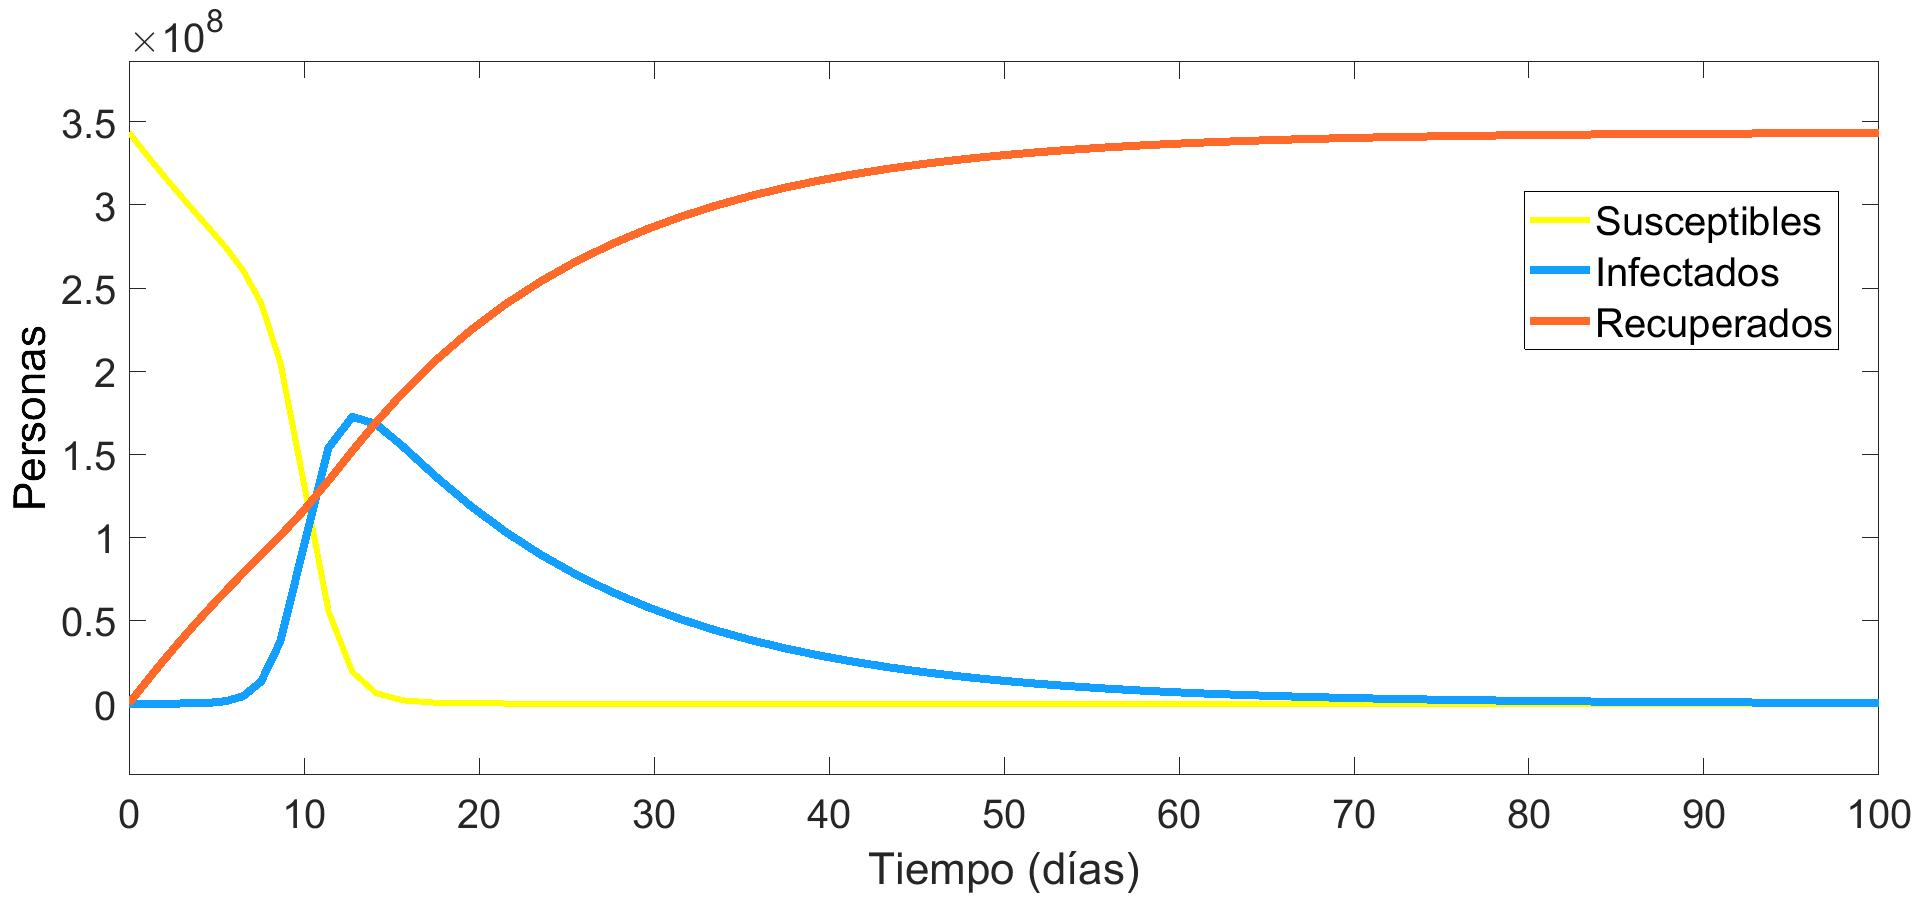
\includegraphics[width=0.9\textwidth]{img/modelo SIRV.jpg}
    \caption{Resultado modelo SIRV con datos reales para el sarampión, con medida de control de vacunación}
    \label{fig:simu saramp vacuna}
    \vspace{0.5cm} % Ajusta el espacio vertical entre la imagen y el texto
\end{figure}

En la gráfica \ref{fig:simu saramp vacuna} las personas susceptibles descienden muy rápido en los primero días, más pronunciado que la simulación sin vacunación. Se debe a que gran parte de los susceptibles son vacunados directamente, lo que reduce la cantidad de personas expuestas al contagio. Prácticamente en los primeros días desaparece el grupo de susceptibles, lo que limita la propagación del virus.
En cuanto a los infectados, aunque se alcanza un pico de infecciones, es más bajo que en la simulación sin vacunación. Se sitúa en torno a 11 millones de infectados, además se produce más temprano, que indica que el brote es más contenido y se disipa más rápido por la inmunidad inducida por la vacunación.
Mientras que el número de recuperados crece rápidamente desde los primeros días. A diferencia del modelo sin vacunación, donde el crecimiento del grupo recuperado dependía únicamente de las personas que superaban la enfermedad, en esta simulación también se incluyen los vacunados, que pasan directamente a este compartimento. Por ello, la curva de recuperados comienza a crecer antes y con mayor pendiente, alcanzando valores más altos en menos tiempo y reflejando una inmunidad colectiva mucho más rápida.

La comparación entre ambas simulaciones muestra claramente que la introducción de la vacunación masiva es altamente efectiva para contener la propagación del sarampión. Reduce significativamente el número de casos, la duración del brote y la exposición de la población susceptible. Esto evidencia la importancia de las campañas de vacunación como herramienta clave de salud pública, especialmente frente a enfermedades con un número básico de reproducción elevado como el sarampión.

\subsection{Comportamiento COVID-19 con vacunación}
Para este modelo, los datos también se han explicado en el apartado de descripción de los datos. Son los mismos que para sin vacunación, lo que pasa que se añade la tasa de vacunación. La figura \ref{fig:Simucov vacunacion} muestra la evolución del sarampión

\begin{figure}[H]
    \centering
    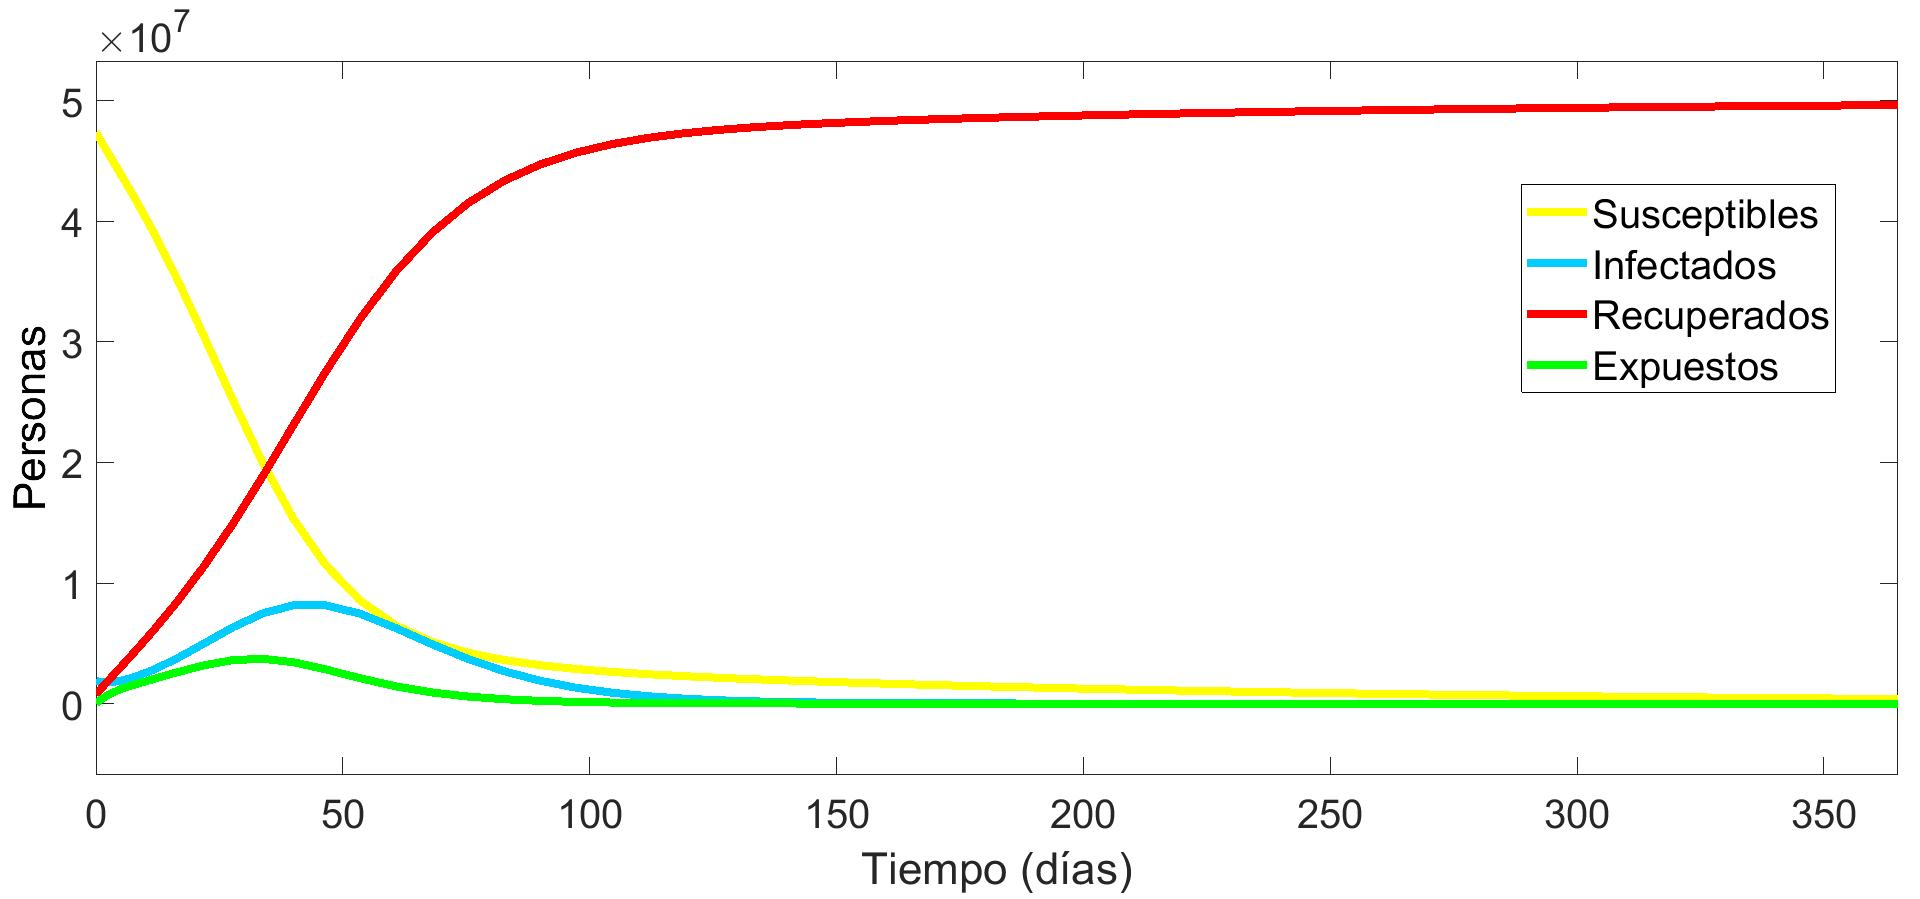
\includegraphics[width=0.9\textwidth]{img/modelo SEIRV.jpg}
    \caption{Resultado modelo SEIRV con datos reales para el COVID-19, con medida de control de vacunación}
    \label{fig:Simucov vacunacion}
    \vspace{0.5cm} % Ajusta el espacio vertical entre la imagen y el texto
\end{figure}

Tras implementar el modelo SEIRV con la incorporación de la vacunación masiva en la población, se puede observar un cambio sustancial en la evolución de la epidemia de COVID-19 respecto al modelo SEIR sin vacunación \ref{fig:Simucov vacunacion}.
En la gráfica obtenida con el modelo SEIRV, se aprecia cómo el número de infectados alcanza un pico considerablemente menor y de menos duración en comparación con la simulación sin vacunación. Este resultado evidencia que la campaña de vacunación contribuye significativamente a reducir la carga máxima del sistema sanitario, evitando un colapso en momentos críticos.
El número de susceptibles disminuye rápidamente debido a dos factores: el contagio y la vacunación. A diferencia del modelo sin vacunación, donde la disminución se debía únicamente a la transmisión del virus, en este caso parte de la población abandona el estado de susceptible al recibir la vacuna y se incorpora directamente al compartimento de recuperados, sin haber pasado por la enfermedad, pero con la misma inmunidad que las personas que han pasado la enfermedad.
La curva de recuperados muestra un crecimiento más rápido y sostenido gracias al efecto de la vacunación, alcanzando antes un número elevado de personas inmunes. Esto acelera la inmunidad colectiva, lo que a su vez disminuye la probabilidad de nuevos contagios en fases posteriores.
Asimismo, la curva de expuestos, representa a aquellos que han estado en contacto con el virus pero aún no son contagiosos, muestra un comportamiento más controlado, evitando una acumulación excesiva de casos latentes como ocurría en la simulación sin vacunación.
Comparando ambos modelos, se concluye que la vacunación tiene un impacto clave en:
\begin{itemize}
    \item Disminuir el número total de personas infectadas.
    \item Reducir la velocidad de propagación.
    \item Limitar el número de personas susceptibles en el tiempo.
    \item Acelerar el final de la epidemia al aumentar rápidamente el número de recuperados.
\end{itemize}	
Estos resultados reflejan de forma cuantitativa cómo una campaña de vacunación masiva, como la que se implementó en España a partir de diciembre de 2020, puede modificar de manera muy significativa la evolución de una pandemia, confirmando la eficacia de esta estrategia como medida de control sanitario.







\section{Discusión}
\textbf{Modelo SI}.
A patrir de las simulaciones de este modelo se puede concluir:
\begin{itemize}
    \item A mayor valor de $\beta$, mayor será la velocidad de propagación de la enfermedad.
    \item Una $\beta$ baja ralentiza el brote, permitiendo una intervención más efectiva.
\end{itemize}

\vspace{2em} 

\textbf{Modelo SI, SIDA/VIH}. Aunque el modelo SI es útil para representar la transmisión crónica del VIH, se trata de una idealización que no refleja completamente la complejidad de su propagación real. El VIH se transmite principalmente por vía sexual, por lo que el riesgo de contagio varía según factores como el comportamiento sexual, el uso de protección, el número de parejas, y el acceso a educación y servicios sanitarios.

El modelo asume una transmisión homogénea en toda la población, pero en la práctica existen grupos con mayor exposición, como trabajadores sexuales o personas que consumen drogas inyectables, lo que introduce una heterogeneidad no contemplada en el modelo.
Además, medidas de prevención como campañas educativas, pruebas diagnósticas o tratamientos antirretrovirales pueden modificar drásticamente la evolución de la epidemia, frenando la propagación. Por ello, aunque el modelo SI proporciona una base teórica útil, sus resultados deben interpretarse con cautela, teniendo en cuenta los múltiples factores sociales y biológicos que influyen en la dinámica del VIH.


\vspace{2em}

\textbf{Modelo SIS}.
Una de las observaciones más relevantes de las simulaciones es que la enfermedad no afecta a toda la población simultáneamente. Los individuos infectados se recuperan y vuelven al estado de susceptibles, creando un flujo continuo entre los dos estados. Este ciclo permite que la enfermedad nunca desaparezca por completo y se estabilice en un equilibrio dinámico.
Por tanto, se puede concluir que:
\begin{itemize}
    \item Si la transmisión supera a la recuperación (beta > gamma), la enfermedad persiste en la población de manera crónica y endémica. En este caso $R_0$ es mayor que 1.
    \item Si la recuperación supera a la transmisión (gamma > beta), la enfermedad tiende a desaparecer con el tiempo. $R_0$ es menor que 1.
\end{itemize}	
Los resultados reflejan que las estrategias para el control o erradicación de enfermedades deben centrarse en: reducir la tasa de transmisión y aumentar la tasa de recuperación. La correcta gestión de estos factores permitirá contener o eliminar enfermedades sin inmunidad permanente, garantizando un mejor estado de salud pública a largo plazo.

\vspace{2em}

\textbf{Modelo SIS, gonorrea}. Proporciona una idealización útil para analizar enfermedades como la gonorrea. Sin embargo, su simplicidad no capta la complejidad del contagio en la vida real.
La gonorrea es una infección de transmisión sexual, y el riesgo de contraerla varía según factores como el comportamiento sexual o el uso de protección. El modelo asume una transmisión homogénea, pero en la práctica existen grupos con mayor riesgo.
Por tanto, aunque el modelo SIS permite una aproximación teórica útil, sus resultados deben interpretarse con precaución. Es necesario complementarlo con un enfoque epidemiológico que tenga en cuenta la diversidad social y conductual para diseñar estrategias de prevención más efectivas y realistas.

\vspace{2em}

\textbf{Modelo SIR}. 	
Una observación importante es que la enfermedad no permanece en equilibrio en la población, a diferencia del modelo SIS. La enfermedad desaparece de forma natural.
Por tanto, se puede concluir que:
\begin{itemize}
    \item Si $\beta$ es alta y $\gamma$ es baja, se alcanzará un pico epidémico más rápido y alto.
    \item Si $\gamma$ es alta o $\beta$ es baja, la propagación será más lenta y es posible que el brote se controle sin llegar a afectar a una gran parte de la población.
    \item En todos los casos donde $R_0$ > 1, el brote se extenderá inicialmente, pero terminará decayendo cuando no queden suficientes susceptibles.
\end{itemize}
Los resultados reflejan la importancia de reducir la tasa de transmisión y aumentar la de recuperación, ya que determinan si la enfermedad provocará una epidemia masiva o se controlará antes de alcanzar un umbral crítico.

\vspace{2em}

\textbf{Modelo SIR, sarampión}.Es útil para representar la dinámica general del sarampión, especialmente por la inmunidad permanente tras la infección. Sin embargo, es una simplificación que no refleja completamente la realidad epidemiológica.
Asume una población homogénea y no considera factores como la distribución geográfica, la edad, el acceso a servicios sanitarios o las intervenciones externas. Tampoco incorpora desigualdades sociales que influyen en la transmisión y el control de la enfermedad.
Por tanto, aunque la simulación reproduce bien el patrón teórico de una epidemia en ausencia de inmunización, sus resultados deben interpretarse con cautela. El modelo debe complementarse con datos reales para diseñar estrategias de salud pública más ajustadas a la realidad.

\vspace{2em}

\textbf{Modelo SIRV, sarampión}. Aunque gran cobertura de vacunación, es importante recordar que esta cifra es el resultado de décadas de esfuerzo en campañas de inmunización.  El modelo, sin embargo, simplifica la realidad al asumir una cobertura alta y constante desde el inicio, sin reflejar diferencias históricas, regionales o de rechazo vacunal.
Aun así, esta idealización es útil desde el punto de vista teórico, ya que permite mostrar cómo la vacunación reduce la población susceptible y previene epidemias, destacando su papel clave en la salud pública. Pese a las limitaciones, el modelo sigue siendo una herramienta eficaz para mostrar el impacto positivo de la vacunación y ayudar a entender su importancia en el control del sarampión.

\vspace{2em}


\textbf{Modelo SIR con regulador PID}.
El uso de un controlador PID mejora la respuesta del sistema frente a una epidemia. A diferencia de las simulaciones sin control, donde las infecciones se mantienen en niveles altos, el PID logra reducir los picos de contagio y acercar el número de infectados al valor deseado. El controlador actúa sobre el parámetro de transmisión 
$\beta$. Así, el modelo controlado se convierte en una herramienta eficaz para analizar y planificar estrategias de contención durante brotes epidémicos.
\vspace{2em}

\textbf{Modelo SEIR}. Tras realizar diversas simulaciones, se ha podido observar cómo la incorporación de un periodo de incubación modifica significativamente la dinámica de propagación 
Se ha comprobado que:
\begin{itemize}
    \item Un valor alto de $\beta$, combinado con un $\sigma$ elevado, conduce a un brote rápido y agresivo, ya que las personas expuestas se convierten rápidamente en infecciosas, alimentando el ciclo de contagio sin apenas retraso.
    \item Cuando $\sigma$ es bajo, es decir, cuando el periodo de incubación es más largo, el crecimiento inicial de los casos se frena. Esto genera una curva más aplanada, aunque el número total de infectados acumulados puede ser similar. El retraso en los contagios retrasa también el pico de infecciones y lo suaviza, facilitando su gestión.
    \item Un $\gamma$ alto (recuperación rápida) reduce tanto la duración como la magnitud del brote. En cambio, una recuperación lenta implica que los infectados permanecen más tiempo en la población, aumentando las posibilidades de contagio y prolongando la epidemia.
\end{itemize}
En cuanto al número básico de reproducción $R_0$, sigue siendo un parámetro esencial para predecir el comportamiento general del sistema. Cuando $R_0$ > 1, la enfermedad se propaga, mientras que si $R_0$ < 1, la infección no puede sostenerse en la población y desaparece.


\vspace{2em}
\textbf{Modelo SEIR, COVID-19}. Idealización matemática que permite estudiar la dinámica de la enfermedad del COVID-19. Su utilidad es reflejar la fase latente previa a la infección activa, lo que le aporta mayor precisión frente a modelos como el SIR.
Sin embargo, asume una población homogénea y no considera factores reales. Tampoco incluye los casos asintomáticos ni la heterogeneidad en los tiempos de incubación, aspectos clave en la propagación del virus.
A pesar de estas limitaciones, el ofrece una herramienta valiosa para analizar de forma cualitativa el comportamiento general del brote. Combinado con datos reales, permite simular escenarios, evaluar intervenciones sanitarias y apoyar el diseño de estrategias de control más eficaces.

\vspace{2em}

\textbf{Modelo SEIRV, COVID-19}. Al asumir una cobertura de vacunación elevada e inmunidad permanente tras la vacunación o recuperación, representa una simplificación teórica que no refleja por completo la complejidad del COVID-19.
La inmunidad frente al COVID-19 puede disminuir con el tiempo y variar según la persona, requiriendo dosis de refuerzo. Además, existen factores que reducen la eficacia de la vacuna, dejando a población vulnerable, incluso con alta cobertura.
El modelo tampoco contempla la aparición de nuevas variantes ni la mortalidad, factores clave en la evolución real de la pandemia. Asumir que todos los infectados se recuperan puede llevar a una subestimación del impacto sanitario.
Pese a estas limitaciones, el modelo SEIRV es útil para visualizar de forma teórica el efecto de la vacunación sobre la dinámica epidémica. Sin embargo, para análisis más precisos y aplicables a la gestión sanitaria, se requieren modelos más complejos que incluyan reinfecciones, pérdida de inmunidad, variantes y mortalidad.